\documentclass{article}\usepackage[]{graphicx}\usepackage[]{color}
%% maxwidth is the original width if it is less than linewidth
%% otherwise use linewidth (to make sure the graphics do not exceed the margin)
\makeatletter
\def\maxwidth{ %
  \ifdim\Gin@nat@width>\linewidth
    \linewidth
  \else
    \Gin@nat@width
  \fi
}
\makeatother

\definecolor{fgcolor}{rgb}{0.345, 0.345, 0.345}
\newcommand{\hlnum}[1]{\textcolor[rgb]{0.686,0.059,0.569}{#1}}%
\newcommand{\hlstr}[1]{\textcolor[rgb]{0.192,0.494,0.8}{#1}}%
\newcommand{\hlcom}[1]{\textcolor[rgb]{0.678,0.584,0.686}{\textit{#1}}}%
\newcommand{\hlopt}[1]{\textcolor[rgb]{0,0,0}{#1}}%
\newcommand{\hlstd}[1]{\textcolor[rgb]{0.345,0.345,0.345}{#1}}%
\newcommand{\hlkwa}[1]{\textcolor[rgb]{0.161,0.373,0.58}{\textbf{#1}}}%
\newcommand{\hlkwb}[1]{\textcolor[rgb]{0.69,0.353,0.396}{#1}}%
\newcommand{\hlkwc}[1]{\textcolor[rgb]{0.333,0.667,0.333}{#1}}%
\newcommand{\hlkwd}[1]{\textcolor[rgb]{0.737,0.353,0.396}{\textbf{#1}}}%
\let\hlipl\hlkwb

\usepackage{framed}
\makeatletter
\newenvironment{kframe}{%
 \def\at@end@of@kframe{}%
 \ifinner\ifhmode%
  \def\at@end@of@kframe{\end{minipage}}%
  \begin{minipage}{\columnwidth}%
 \fi\fi%
 \def\FrameCommand##1{\hskip\@totalleftmargin \hskip-\fboxsep
 \colorbox{shadecolor}{##1}\hskip-\fboxsep
     % There is no \\@totalrightmargin, so:
     \hskip-\linewidth \hskip-\@totalleftmargin \hskip\columnwidth}%
 \MakeFramed {\advance\hsize-\width
   \@totalleftmargin\z@ \linewidth\hsize
   \@setminipage}}%
 {\par\unskip\endMakeFramed%
 \at@end@of@kframe}
\makeatother

\definecolor{shadecolor}{rgb}{.97, .97, .97}
\definecolor{messagecolor}{rgb}{0, 0, 0}
\definecolor{warningcolor}{rgb}{1, 0, 1}
\definecolor{errorcolor}{rgb}{1, 0, 0}
\newenvironment{knitrout}{}{} % an empty environment to be redefined in TeX

\usepackage{alltt}

\usepackage[utf8]{inputenc}
\usepackage{hyperref}
\usepackage{booktabs}
\usepackage{longtable}
\usepackage{array}
\usepackage{multirow}
\usepackage[table]{xcolor}
\usepackage{wrapfig}
\usepackage{float}
\usepackage{colortbl}
\usepackage{pdflscape}
\usepackage{tabu}
\usepackage{threeparttable}
\usepackage{threeparttablex}
\usepackage[normalem]{ulem}
\usepackage{makecell}

\hypersetup{
    linktocpage,
    colorlinks=true, 
    linkcolor=blue,
    citecolor=blue,
    filecolor=blue,
    urlcolor=blue
}
\IfFileExists{upquote.sty}{\usepackage{upquote}}{}
\begin{document}


  
\title{Heatschock Arrays}
\author{Elisabet Tintó, Lucas Michel Todó}
\maketitle
\tableofcontents
\clearpage

%%%%------------------------------------------------FC------------------------------------------------%%%%

\section{Imputed FC}


\subsection{10E FC}
\begin{knitrout}
\definecolor{shadecolor}{rgb}{0.969, 0.969, 0.969}\color{fgcolor}\begin{table}[H]
\centering\rowcolors{2}{gray!6}{white}

\resizebox{\linewidth}{!}{
\begin{tabular}{rrrrll}
\hiderowcolors
\toprule
s10E\_T1\_HS & s10E\_T2\_HS & s10E\_T3\_HS & Max\_Dif & Gene & Annot\\
\midrule
\showrowcolors
2.0489945 & 4.0265577 & 2.7637695 & 4.026558 & PF3D7\_0818900 & heat shock prot. 70\\
-1.7218645 & -3.8935602 & 0.2723678 & -3.893560 & PF3D7\_1428000 & cvd. Pl. memb. prot. ukwn. func.\\
1.2330183 & 3.6222511 & 2.8090811 & 3.622251 & PF3D7\_1000600 & rifin\\
-2.6150582 & -3.4433569 & 0.3468610 & -3.443357 & S2-type\_28S:rRNA & NA\\
-1.9884922 & -3.3929230 & -0.6069939 & -3.392923 & PF3D7\_0112600 & unspecified product\\
\addlinespace
-2.0439641 & -3.3074306 & 0.3950818 & -3.307431 & PF3D7\_1455900 & polyprenol reductase put.\\
-1.3421985 & -3.2800100 & 0.0124447 & -3.280010 & PF3D7\_0717000 & cvd. Pl. memb. prot. ukwn. func.\\
-1.6829756 & -3.2617931 & 0.9056299 & -3.261793 & PF3D7\_0622700 & cvd. Pl. memb. prot. ukwn. func.\\
1.8267402 & 3.1565584 & 1.2542698 & 3.156558 & PF3D7\_1421800 & cvd. Pl. prot. ukwn. func.\\
-1.6207045 & -3.1124710 & 0.3854057 & -3.112471 & PF3D7\_0911000 & phosphatidylinositol N-acetylglucosaminyltransferase put.\\
\addlinespace
NA & NA & -3.0633088 & -3.063309 & PF14TR007 & NA\\
-1.3878045 & -3.0022915 & 0.6412622 & -3.002292 & PF3D7\_0929900 & cvd. Pl. prot. ukwn. func.\\
-1.3984653 & -2.8614779 & 0.0744639 & -2.861478 & PF3D7\_0523500 & dynein light chain Tctex-type put.\\
-1.5566419 & -2.8224296 & -0.1544318 & -2.822430 & PF3D7\_0627200 & myosin light chain put.\\
-0.9800127 & -2.8060897 & -0.0950306 & -2.806090 & PF3D7\_0414200 & calmodulin-like prot.\\
\addlinespace
1.0834900 & 2.7624204 & 0.9954510 & 2.762420 & PF3D7\_0214300 & cvd. Pl. prot. ukwn. func.\\
2.7529274 & 0.0941567 & -0.1863445 & 2.752927 & PF3D7\_1314800 & ubiquitin-like prot. put.\\
1.2478092 & 2.7240805 & 1.0579105 & 2.724080 & PF3D7\_0404600 & cvd. Pl. memb. prot. ukwn. func.\\
-1.0022730 & -2.6543406 & 1.0460634 & -2.654341 & PF3D7\_1322800 & cvd. Pl. prot. ukwn. func.\\
0.6521131 & 2.6276509 & 1.8115100 & 2.627651 & PF3D7\_0525000 & zinc finger prot. put.\\
\addlinespace
0.9531122 & 2.5804698 & 0.2909951 & 2.580470 & PF3D7\_1362700 & cvd. Pl. prot. ukwn. func.\\
1.1187591 & 2.5662126 & 1.3217427 & 2.566213 & PF3D7\_0220300 & Pl. xptd. prot. ukwn. func.\\
-1.3852968 & -2.5657303 & 0.2571554 & -2.565730 & PF3D7\_0613200 & cvd. Pl. prot. ukwn. func.\\
-0.8289211 & -2.5057559 & 0.2416806 & -2.505756 & PF3D7\_1433600 & signal peptidase complex subunit SPC1 put.\\
0.4870453 & 2.4677876 & 2.1483594 & 2.467788 & PF3D7\_1038700 & Pl. xptd. prot. ukwn. func.\\
\addlinespace
-0.4539304 & 0.8211792 & 2.4543858 & 2.454386 & PF3D7\_0324100 & Pfmc-2TM Maurer's cleft two transmemb. prot.\\
0.6091590 & 2.4531509 & 1.6318496 & 2.453151 & BSD & NA\\
-0.9269817 & -2.4487225 & 0.0859541 & -2.448723 & PF3D7\_1135000 & PQ-loop repeat-containing prot. unspecified product\\
-0.9352453 & -2.4359463 & -0.2882011 & -2.435946 & PF3D7\_0729200 & 1-cys peroxiredoxin\\
-0.7109644 & -0.9582562 & 2.4359055 & 2.435906 & PF3D7\_0524200 & cvd. Pl. memb. prot. ukwn. func.\\
\addlinespace
-0.6880042 & -2.4299811 & -0.5552725 & -2.429981 & PF3D7\_0323000 & translation machinery-associated prot. 7 put.\\
0.8225018 & 1.8692184 & 2.4227689 & 2.422769 & PF3D7\_0800700 & surface-associated interspersed prot. 8.3 (SURFIN 8.3)\\
-1.1773975 & -2.4011238 & 0.1421178 & -2.401124 & PF3D7\_1371500 & probable prot. ukwn. func.\\
0.1143743 & 2.3856525 & 1.9254568 & 2.385652 & PF3D7\_1201100 & RESA-like prot. with PHIST and DnaJ domains\\
-0.8600038 & -2.3812869 & 0.3315026 & -2.381287 & PF3D7\_0912700 & cvd. Pl. prot. ukwn. func.\\
\addlinespace
-0.5896510 & -2.3785127 & 0.4246107 & -2.378513 & PF3D7\_1413300 & cvd. Pl. prot. ukwn. func.\\
-0.3469780 & 0.3254741 & 2.3646003 & 2.364600 & PF3D7\_1237300 & cvd. Pl. prot. ukwn. func.\\
0.5498747 & 1.8887517 & 2.3534550 & 2.353455 & PF3D7\_0404500 & 6-cysteine prot.\\
-1.3798491 & -2.3159824 & 1.8946139 & -2.315982 & PF3D7\_0513700 & secreted ookinete prot. put.\\
-0.5500801 & -2.3145427 & -0.3863081 & -2.314543 & PF3D7\_1447700 & cvd. Pl. prot. ukwn. func.\\
\addlinespace
-0.7214122 & -2.2885964 & -0.6557671 & -2.288596 & PF3D7\_1459300 & OPA3-like prot. put.\\
-0.9626105 & -2.2796311 & -0.3062433 & -2.279631 & PF3D7\_1463600 & cvd. Pl. prot. ukwn. func.\\
-1.1915921 & -2.2794752 & -0.2588739 & -2.279475 & PF3D7\_0112400 & unspecified product\\
-0.9207716 & -1.7445386 & -2.2727826 & -2.272783 & PF3D7\_1373000 & rifin\\
-1.3589828 & -2.2670347 & 0.8246955 & -2.267035 & PF3D7\_0618600 & rhomboid protease ROM10\\
\addlinespace
-2.2648826 & -2.0425870 & -1.4067897 & -2.264883 & PF3D7\_0800800 & Pl. xptd. prot. (hyp7) ukwn. func.\\
0.6381268 & 2.2531239 & 1.1319811 & 2.253124 & PF3D7\_0113400 & Pl. xptd. prot. ukwn. func.\\
-1.0199383 & -2.2500155 & 0.3172939 & -2.250015 & PF3D7\_0414300 & Rab5-interacting prot. put.\\
0.9314392 & 2.2474121 & 1.0281318 & 2.247412 & PF3D7\_1236200 & cvd. Pl. prot. ukwn. func.\\
-1.0373801 & -2.2326496 & -1.3494395 & -2.232650 & PF3D7\_0936100 & early transcribed memb. prot.\\
\bottomrule
\end{tabular}}
\rowcolors{2}{white}{white}
\end{table}


\end{knitrout}
\clearpage
\subsection{10G FC}
\begin{knitrout}
\definecolor{shadecolor}{rgb}{0.969, 0.969, 0.969}\color{fgcolor}\begin{table}[H]
\centering\rowcolors{2}{gray!6}{white}

\resizebox{\linewidth}{!}{
\begin{tabular}{rrrrll}
\hiderowcolors
\toprule
s10G\_T1\_HS & s10G\_T2\_HS & s10G\_T3\_HS & Max\_Dif & Gene & Annot\\
\midrule
\showrowcolors
2.1137451 & 4.2991723 & 4.9279716 & 4.927972 & PF3D7\_1201100 & RESA-like prot. with PHIST and DnaJ domains\\
2.6347191 & 4.4548988 & 4.8855375 & 4.885537 & PF3D7\_0425900 & rifin\\
-1.3298695 & -4.5527720 & -2.2619124 & -4.552772 & PF3D7\_0211000 & unspecified product\\
1.9378205 & 3.9765343 & 4.5024441 & 4.502444 & Pfa\_npcR\_6502a & NA\\
3.0149005 & 3.8700142 & 4.0953486 & 4.095349 & PF3D7\_1000600 & rifin\\
\addlinespace
-0.0436569 & 1.5137139 & 4.0231735 & 4.023174 & PF3D7\_1479000 & acyl-CoA synthetase\\
1.4033747 & 3.3103404 & 3.9649935 & 3.964993 & PF3D7\_1200200 & rifin\\
1.1564351 & 2.7860372 & 3.8797703 & 3.879770 & Pfa\_raR\_7295 & NA\\
-0.4848050 & 1.5423599 & 3.8648579 & 3.864858 & PF3D7\_1478900 & unspecified product\\
1.3015494 & 3.3485580 & 3.8227606 & 3.822761 & PF3D7\_0220500 & Pl. xptd. prot. (hyp2) ukwn. func.\\
\addlinespace
-1.8063928 & -3.7768931 & -2.9373609 & -3.776893 & PF3D7\_0523500 & dynein light chain Tctex-type put.\\
-1.4848834 & -3.7246744 & -2.8094441 & -3.724674 & PF3D7\_1371500 & probable prot. ukwn. func.\\
1.4217156 & 3.2457568 & 3.6716633 & 3.671663 & BSD & NA\\
-1.7510847 & -3.6173576 & -2.4031305 & -3.617358 & PF3D7\_1428000 & cvd. Pl. memb. prot. ukwn. func.\\
-3.5057700 & -3.2247349 & 0.0167300 & -3.505770 & S2-type\_28S:rRNA & NA\\
\addlinespace
0.0457444 & 2.1141881 & 3.4928105 & 3.492811 & PF3D7\_1104900 & calcium/calmodulin-dependent prot. kinase put.\\
-0.5135120 & -3.4531676 & -2.3356841 & -3.453168 & PF3D7\_0304800 & cvd. Pl. memb. prot. ukwn. func.\\
1.1332030 & 3.0559121 & 3.3941579 & 3.394158 & PF3D7\_0830500 & sporozoite and liver stage tryptophan-rich prot. put.\\
0.9869742 & 2.9827184 & 3.3563964 & 3.356396 & PF3D7\_1473700 & nucleoporin NUP116/NSP116 put.\\
2.0091358 & 2.7803212 & 3.3537782 & 3.353778 & PF3D7\_0919200 & PPPDE peptidase put.\\
\addlinespace
0.9201151 & 2.9630996 & 3.3395569 & 3.339557 & PF3D7\_1455300 & cvd. Pl. prot. ukwn. func.\\
1.3342481 & 3.1096949 & 3.3372747 & 3.337275 & PF3D7\_1461800 & cvd. Pl. prot. ukwn. func.\\
0.9638254 & 2.7438073 & 3.3338683 & 3.333868 & PF3D7\_0115600 & rifin\\
-0.9007556 & -3.3322740 & -2.7956473 & -3.332274 & PF3D7\_1447700 & cvd. Pl. prot. ukwn. func.\\
-2.1561557 & -3.3289434 & -2.8495299 & -3.328943 & PF3D7\_0911500 & cvd. Pl. prot. ukwn. func.\\
\addlinespace
-2.0639038 & -3.3133003 & -2.4818534 & -3.313300 & PF3D7\_1455900 & polyprenol reductase put.\\
0.9461254 & 3.0010464 & 3.2978560 & 3.297856 & PF3D7\_1300200 & rifin\\
-2.5060113 & -3.2883457 & -2.0785061 & -3.288346 & PF3D7\_0622700 & cvd. Pl. memb. prot. ukwn. func.\\
2.0435174 & 3.1597876 & 3.2399103 & 3.239910 & PF3D7\_1327300 & cvd. Pl. prot. ukwn. func.\\
-1.0126413 & -3.1831313 & -2.4891014 & -3.183131 & PF3D7\_1442800 & cvd. Pl. prot. ukwn. func.\\
\addlinespace
1.1244585 & 3.1824766 & 3.0773001 & 3.182477 & PF3D7\_0418600 & regulator of chromosome condensation put.\\
-0.6657867 & -3.1754078 & -2.3003331 & -3.175408 & PF3D7\_0612300 & transmemb. prot. 234 put.\\
-1.6523152 & -3.1702565 & -2.4312476 & -3.170256 & PF3D7\_1138900 & unspecified product\\
-1.1460425 & -3.1580070 & -2.9965295 & -3.158007 & PF3D7\_0414200 & calmodulin-like prot.\\
-2.8134191 & -3.1400926 & -2.3479327 & -3.140093 & PF3D7\_0112600 & unspecified product\\
\addlinespace
0.5806812 & 2.1703357 & 3.1307881 & 3.130788 & Pfa\_rasR\_6152b & NA\\
1.0002653 & 3.1290953 & 3.1096016 & 3.129095 & PF3D7\_0424500 & serine/threonine prot. kinase FIKK family\\
-0.7602257 & 0.3923218 & 3.1160955 & 3.116096 & PF14TR011 & NA\\
-0.0854555 & 3.0797745 & 2.4525542 & 3.079775 & PF3D7\_0425200 & Pl. xptd. prot. (hyp15) ukwn. func.\\
-0.7019923 & -3.0575793 & -2.5612616 & -3.057579 & PF3D7\_0531200 & ribosomal prot. S16 mitochondrial put.\\
\addlinespace
0.7540290 & 2.3200485 & 3.0542948 & 3.054295 & PF3D7\_0702100 & Pl. xptd. prot. (PHISTb) ukwn. func. pseudo\\
1.1361720 & 2.4939047 & 3.0444175 & 3.044418 & PF3D7\_0401800 & Pl. xptd. prot. (PHISTb) ukwn. func.\\
-2.1308832 & -3.0369508 & -2.3467176 & -3.036951 & PF3D7\_0929900 & cvd. Pl. prot. ukwn. func.\\
-1.2979217 & -3.0258756 & -2.6800888 & -3.025876 & PF3D7\_0920300 & cvd. Pl. prot. ukwn. func.\\
3.0036935 & NA & 0.5200563 & 3.003693 & ETG10\_13482 & NA\\
\addlinespace
0.2135770 & 2.1148377 & 2.9953831 & 2.995383 & PF3D7\_0931300 & cvd. Pl. prot. ukwn. func.\\
-1.2072390 & -2.9910360 & -2.6865723 & -2.991036 & PF3D7\_1415500 & cvd. Pl. memb. prot. ukwn. func.\\
0.0233773 & 2.1999542 & 2.9807958 & 2.980796 & PF3D7\_0701900 & Pl. xptd. prot. ukwn. func.\\
0.4493020 & 2.6346493 & 2.9774535 & 2.977454 & Pfa\_rasR\_6152a & NA\\
0.9473589 & 2.5585782 & 2.9303477 & 2.930348 & PF3D7\_0902500 & serine/threonine prot. kinase FIKK family\\
\bottomrule
\end{tabular}}
\rowcolors{2}{white}{white}
\end{table}


\end{knitrout}
\clearpage
\subsection{EK0 FC}
\begin{knitrout}
\definecolor{shadecolor}{rgb}{0.969, 0.969, 0.969}\color{fgcolor}\begin{table}[H]
\centering\rowcolors{2}{gray!6}{white}

\resizebox{\linewidth}{!}{
\begin{tabular}{rrrrll}
\hiderowcolors
\toprule
EK0\_T1\_HS & EK0\_T2\_HS & EK0\_T3\_HS & Max\_Dif & Gene & Annot\\
\midrule
\showrowcolors
3.8023938 & 4.8569453 & 4.692690 & 4.856945 & PF3D7\_1201100 & RESA-like prot. with PHIST and DnaJ domains\\
-1.9416306 & -4.2440483 & -4.782000 & -4.782000 & PF3D7\_0211000 & unspecified product\\
1.9045315 & 2.5509136 & 4.638035 & 4.638035 & Pfa\_raR\_7295 & NA\\
-2.6191721 & -4.5922710 & -3.797023 & -4.592271 & PF3D7\_0523500 & dynein light chain Tctex-type put.\\
3.0829661 & 4.5840501 & 3.502010 & 4.584050 & PF3D7\_1301200 & GBPH2 prot.\\
\addlinespace
-1.7539348 & -4.3045094 & -3.829557 & -4.304509 & PF3D7\_1442800 & cvd. Pl. prot. ukwn. func.\\
-1.6471473 & -2.9354249 & -4.289994 & -4.289994 & PF3D7\_0612300 & transmemb. prot. 234 put.\\
-2.2993027 & -4.2293721 & -3.827649 & -4.229372 & PF3D7\_0911500 & cvd. Pl. prot. ukwn. func.\\
2.3895092 & 3.4186546 & 4.196898 & 4.196898 & PF3D7\_0220500 & Pl. xptd. prot. (hyp2) ukwn. func.\\
-2.2256092 & -3.9418175 & -4.064436 & -4.064436 & PF3D7\_1371500 & probable prot. ukwn. func.\\
\addlinespace
-1.4716560 & -4.0427812 & -3.727419 & -4.042781 & PF3D7\_1243200 & cvd. Pl. prot. ukwn. func.\\
-2.2013572 & -2.2424364 & -4.034055 & -4.034055 & PF3D7\_1138900 & unspecified product\\
2.9867359 & 3.1270593 & 3.965262 & 3.965262 & Pfa\_npcR\_6502a & NA\\
2.7148473 & 3.6833436 & 3.914220 & 3.914220 & BSD & NA\\
2.8828779 & 3.7149530 & 3.866368 & 3.866368 & PF3D7\_1200200 & rifin\\
\addlinespace
3.5422016 & 3.8330021 & 3.562946 & 3.833002 & PF3D7\_1000600 & rifin\\
3.2599498 & 3.8277464 & 3.775691 & 3.827746 & PF3D7\_1300200 & rifin\\
-2.3425589 & -3.6534078 & -3.422572 & -3.653408 & PF3D7\_1415500 & cvd. Pl. memb. prot. ukwn. func.\\
-1.1344729 & -3.0483879 & -3.621073 & -3.621073 & PF3D7\_0715700 & cvd. Pl. prot. ukwn. func.\\
2.3225763 & 3.1651720 & 3.608397 & 3.608397 & PF3D7\_1473700 & nucleoporin NUP116/NSP116 put.\\
\addlinespace
-1.5404627 & -3.5764164 & -2.827631 & -3.576416 & PF3D7\_0531200 & ribosomal prot. S16 mitochondrial put.\\
-1.7908769 & -2.9899371 & -3.427631 & -3.427631 & PF3D7\_1428000 & cvd. Pl. memb. prot. ukwn. func.\\
2.0581731 & 2.8904910 & 3.371153 & 3.371153 & PF3D7\_0830500 & sporozoite and liver stage tryptophan-rich prot. put.\\
-1.7929202 & -3.2893443 & -3.314578 & -3.314578 & PF3D7\_1447700 & cvd. Pl. prot. ukwn. func.\\
-2.0022204 & -3.2810434 & -3.309032 & -3.309032 & PF3D7\_1459300 & OPA3-like prot. put.\\
\addlinespace
0.6285579 & 0.9056818 & 3.289550 & 3.289550 & PF3D7\_0726200 & serine/threonine prot. kinase FIKK family\\
-1.1327561 & -3.2863665 & -2.237896 & -3.286367 & PF3D7\_0420500 & cvd. Pl. prot. ukwn. func.\\
-1.4082491 & -2.7197976 & -3.284616 & -3.284616 & PF3D7\_0111700 & cvd. Pl. prot. ukwn. func.\\
-1.5023009 & -2.4758748 & -3.245238 & -3.245238 & PF3D7\_1129800 & cvd. Pl. prot. ukwn. func.\\
1.8234852 & 2.8196199 & 3.212838 & 3.212838 & PF3D7\_1016500 & Pl. xptd. prot. (PHISTc) ukwn. func.\\
\addlinespace
0.8527512 & 2.1333440 & 3.207891 & 3.207891 & PF3D7\_0726100 & Pl. xptd. prot. ukwn. func.\\
1.7393624 & 2.8384464 & 3.186994 & 3.186994 & PF3D7\_1455300 & cvd. Pl. prot. ukwn. func.\\
-2.5140261 & -3.1742956 & -3.117327 & -3.174296 & PF3D7\_0622700 & cvd. Pl. memb. prot. ukwn. func.\\
-1.3762392 & -2.8846323 & -3.172797 & -3.172797 & PF3D7\_1322800 & cvd. Pl. prot. ukwn. func.\\
1.6189063 & 2.5768360 & 3.122261 & 3.122261 & PF3D7\_1327300 & cvd. Pl. prot. ukwn. func.\\
\addlinespace
0.6551133 & 3.1165244 & 2.958353 & 3.116524 & PF3D7\_1000500 & rifin\\
-2.2594348 & -3.0964218 & -2.469610 & -3.096422 & PF3D7\_1474700 & prot. kinase put.\\
-2.9305255 & -2.9541177 & -3.074790 & -3.074790 & PF3D7\_1018400 & cvd. Pl. prot. ukwn. func.\\
1.4200407 & 2.0950576 & 3.071462 & 3.071462 & PF3D7\_1362700 & cvd. Pl. prot. ukwn. func.\\
-1.9342017 & -3.0714373 & -2.481436 & -3.071437 & PF3D7\_0303600 & plasmoredoxin\\
\addlinespace
-1.7850804 & -3.0144346 & -2.845174 & -3.014435 & PF3D7\_0612400 & cvd. Pl. prot. ukwn. func.\\
1.9088095 & 3.0079359 & 2.782675 & 3.007936 & PF3D7\_1226100 & haloacid dehalogenase-like hydrolase put.\\
1.3603219 & 2.3945868 & 2.996161 & 2.996161 & PF3D7\_1000200 & rifin\\
1.3619715 & 2.3611783 & 2.987410 & 2.987410 & PF3D7\_0315600 & zinc finger prot. put.\\
1.7961729 & 2.9766919 & 1.865438 & 2.976692 & PF3D7\_0832100 & rifin pseudo\\
\addlinespace
1.7493615 & 2.7702028 & 2.955449 & 2.955449 & PF3D7\_1461800 & cvd. Pl. prot. ukwn. func.\\
1.1986903 & 2.6384073 & 2.948113 & 2.948113 & PF3D7\_0701900 & Pl. xptd. prot. ukwn. func.\\
-1.1954013 & -2.0072608 & -2.932215 & -2.932215 & PF3D7\_1346600 & cvd. Pl. prot. ukwn. func.\\
-1.4459350 & -2.6859144 & -2.930878 & -2.930878 & PF3D7\_0625700 & cvd. Pl. prot. ukwn. func.\\
-1.4581395 & -2.9126340 & -2.493292 & -2.912634 & PF3D7\_0920300 & cvd. Pl. prot. ukwn. func.\\
\bottomrule
\end{tabular}}
\rowcolors{2}{white}{white}
\end{table}


\end{knitrout}
\clearpage


%%%%------------------------------------------------VENNS------------------------------------------------%%%%

\section{Venn Diagrams}

\subsection{Max.FC (any timepoint) $>3$ FC}
\subsubsection{Up-regulated}

\begin{knitrout}
\definecolor{shadecolor}{rgb}{0.969, 0.969, 0.969}\color{fgcolor}\begin{kframe}
\begin{verbatim}
## (polygon[GRID.polygon.1], polygon[GRID.polygon.2], polygon[GRID.polygon.3], polygon[GRID.polygon.4], polygon[GRID.polygon.5], polygon[GRID.polygon.6], text[GRID.text.7], text[GRID.text.8], text[GRID.text.9], text[GRID.text.10], text[GRID.text.11], text[GRID.text.12], text[GRID.text.13], text[GRID.text.14], text[GRID.text.15], text[GRID.text.16])
\end{verbatim}
\end{kframe}

{\centering 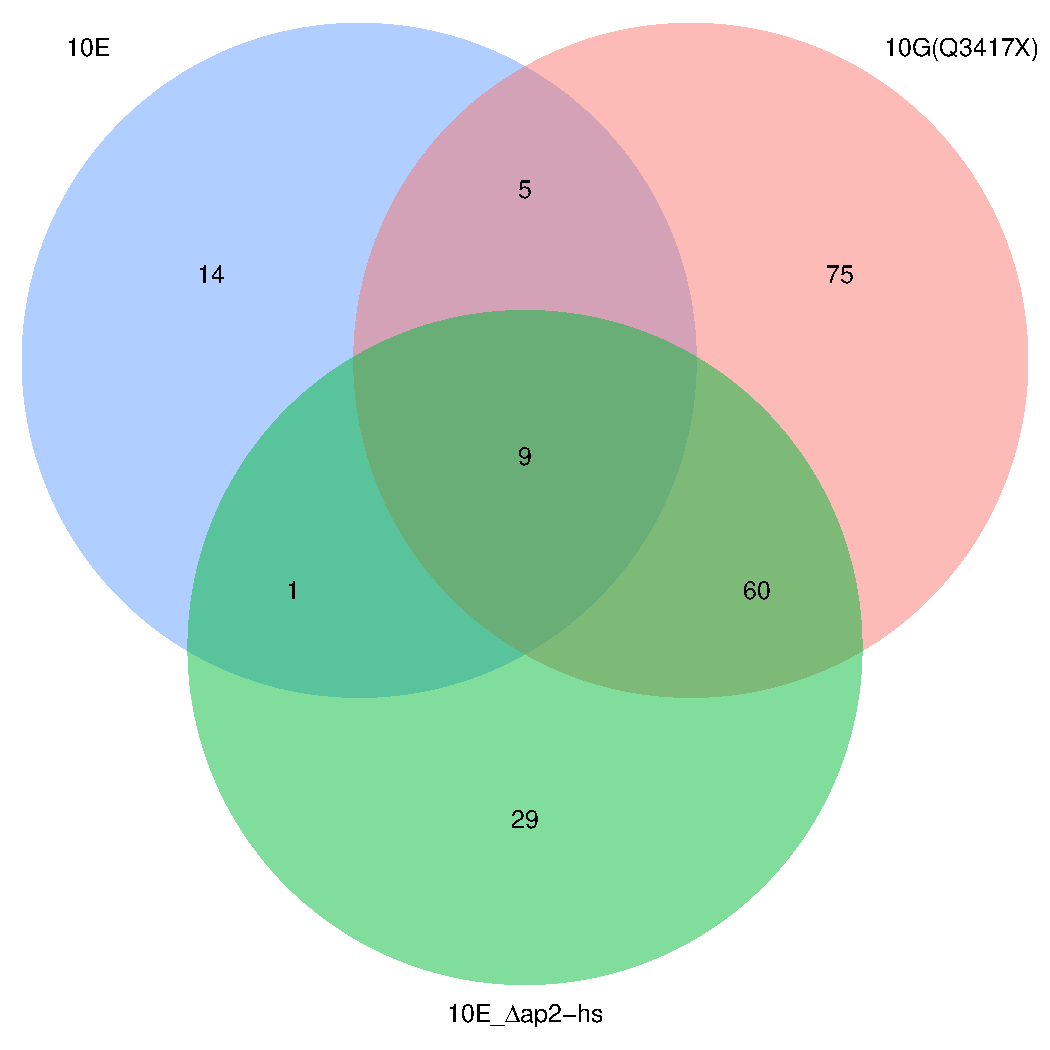
\includegraphics[width=1\linewidth,height=.4\textheight]{figure/minimal-venn_alltimes_3fc_up_venn-1} 

}



\end{knitrout}
\begin{knitrout}
\definecolor{shadecolor}{rgb}{0.969, 0.969, 0.969}\color{fgcolor}

{\centering 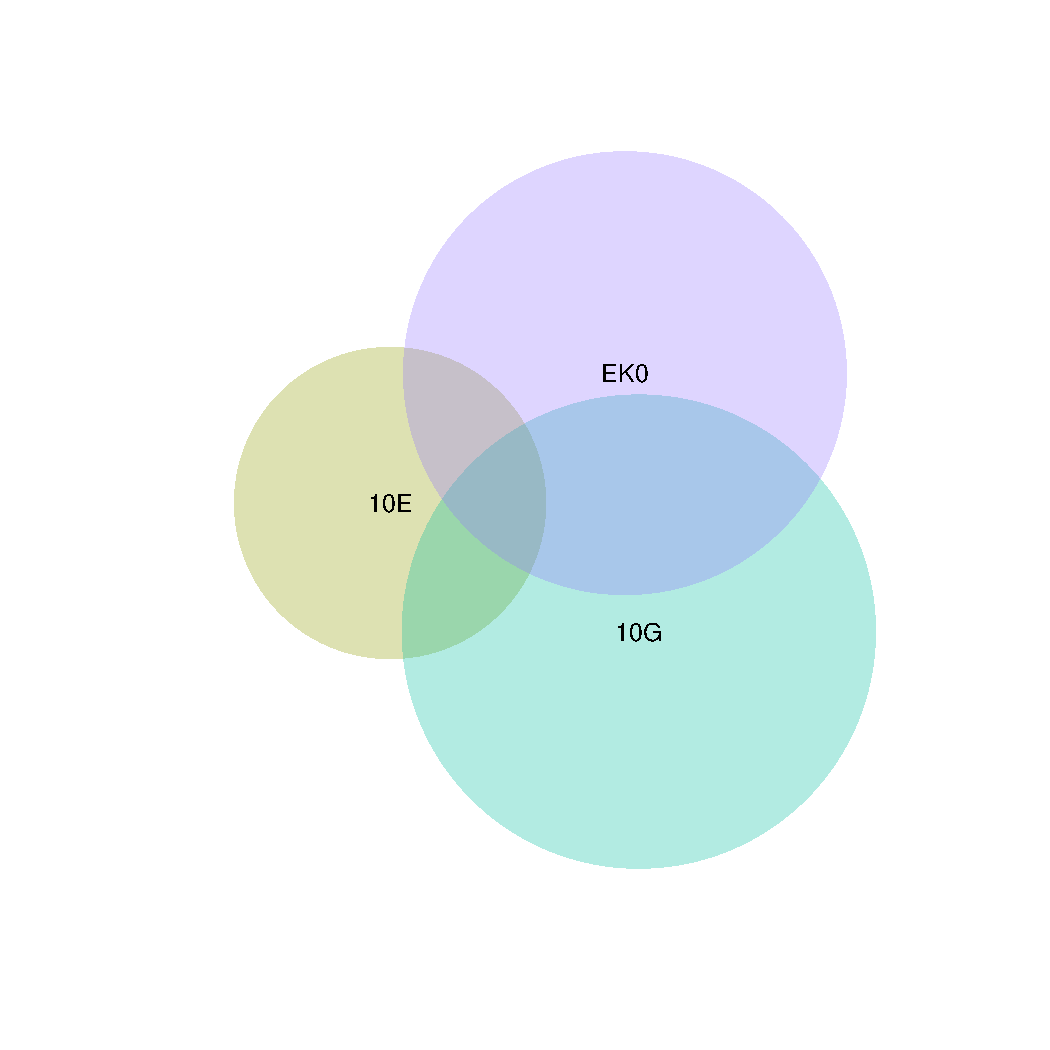
\includegraphics[width=1\linewidth,height=.4\textheight]{figure/minimal-venn_alltimes_3fc_up_euler-1} 

}



\end{knitrout}
\clearpage
\subsubsection{Down-regulated}

\begin{knitrout}
\definecolor{shadecolor}{rgb}{0.969, 0.969, 0.969}\color{fgcolor}\begin{kframe}
\begin{verbatim}
## (polygon[GRID.polygon.17], polygon[GRID.polygon.18], polygon[GRID.polygon.19], polygon[GRID.polygon.20], polygon[GRID.polygon.21], polygon[GRID.polygon.22], text[GRID.text.23], text[GRID.text.24], text[GRID.text.25], text[GRID.text.26], text[GRID.text.27], text[GRID.text.28], text[GRID.text.29], text[GRID.text.30], text[GRID.text.31], text[GRID.text.32])
\end{verbatim}
\end{kframe}

{\centering 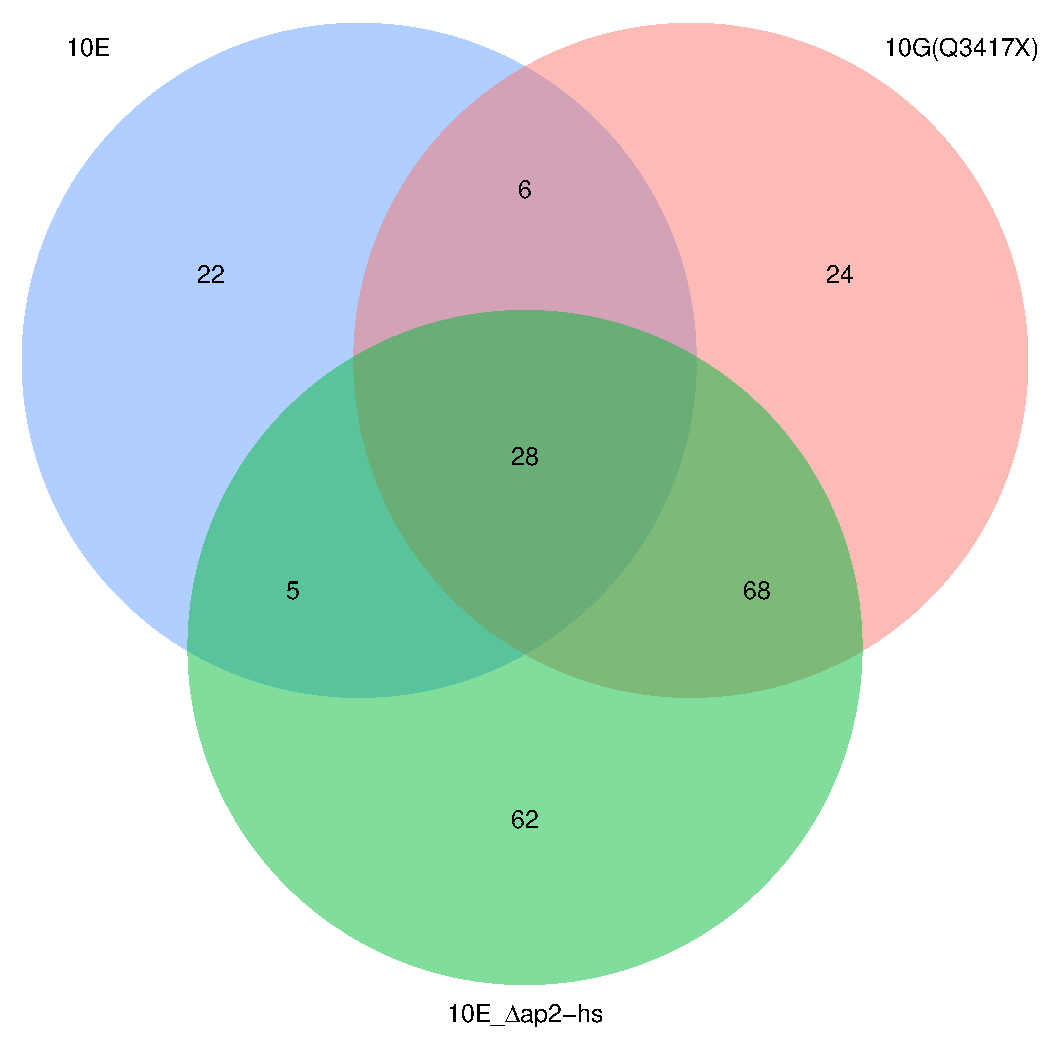
\includegraphics[width=1\linewidth,height=.4\textheight]{figure/minimal-venn_alltimes_3fc_down_venn-1} 

}



\end{knitrout}
\begin{knitrout}
\definecolor{shadecolor}{rgb}{0.969, 0.969, 0.969}\color{fgcolor}

{\centering 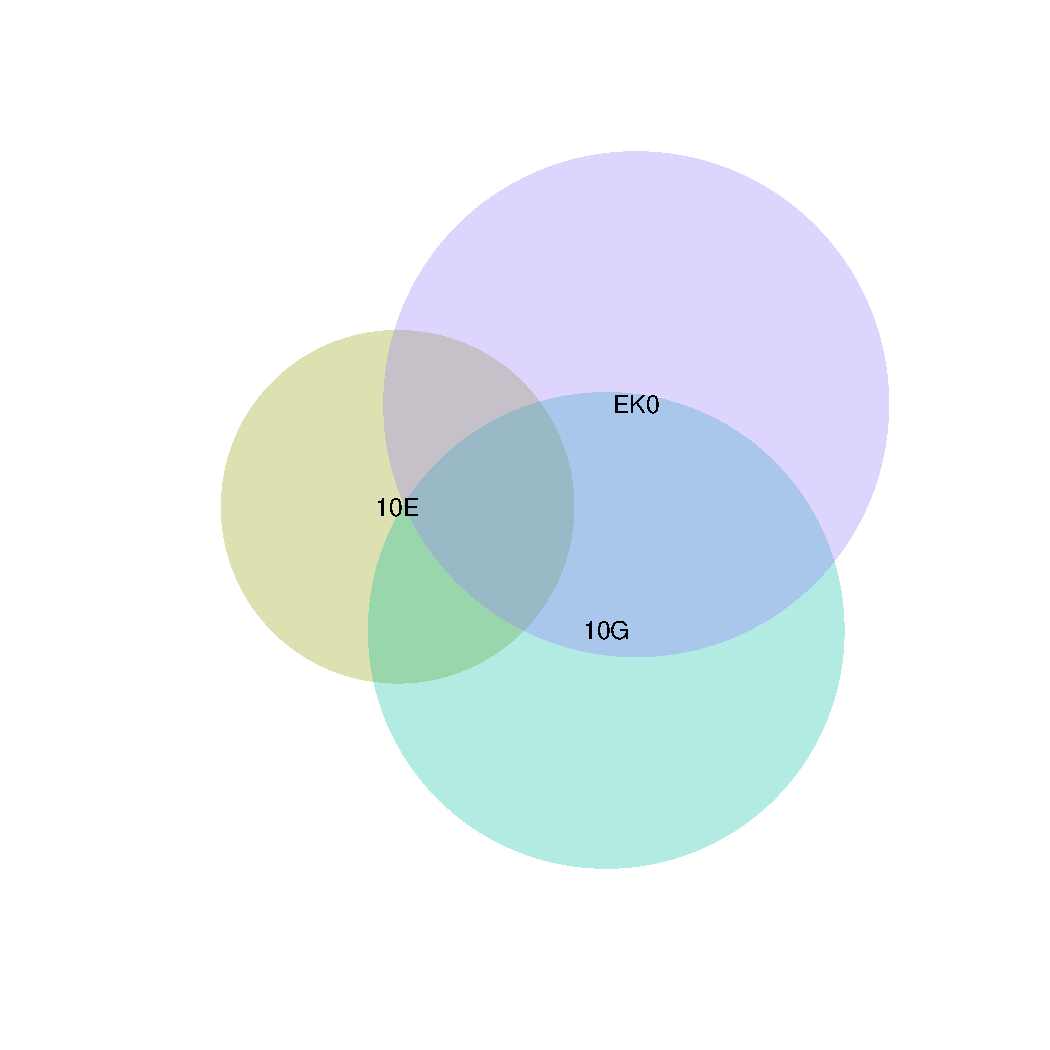
\includegraphics[width=1\linewidth,height=.4\textheight]{figure/minimal-venn_alltimes_3fc_down_euler-1} 

}



\end{knitrout}
\clearpage

\subsection{Max.FC T1 $>3$ FC}
\subsubsection{Up-regulated}

\begin{knitrout}
\definecolor{shadecolor}{rgb}{0.969, 0.969, 0.969}\color{fgcolor}\begin{kframe}
\begin{verbatim}
## (polygon[GRID.polygon.33], polygon[GRID.polygon.34], polygon[GRID.polygon.35], polygon[GRID.polygon.36], polygon[GRID.polygon.37], polygon[GRID.polygon.38], text[GRID.text.39], text[GRID.text.40], text[GRID.text.41], text[GRID.text.42], text[GRID.text.43], text[GRID.text.44], text[GRID.text.45], text[GRID.text.46], text[GRID.text.47], text[GRID.text.48])
\end{verbatim}
\end{kframe}

{\centering 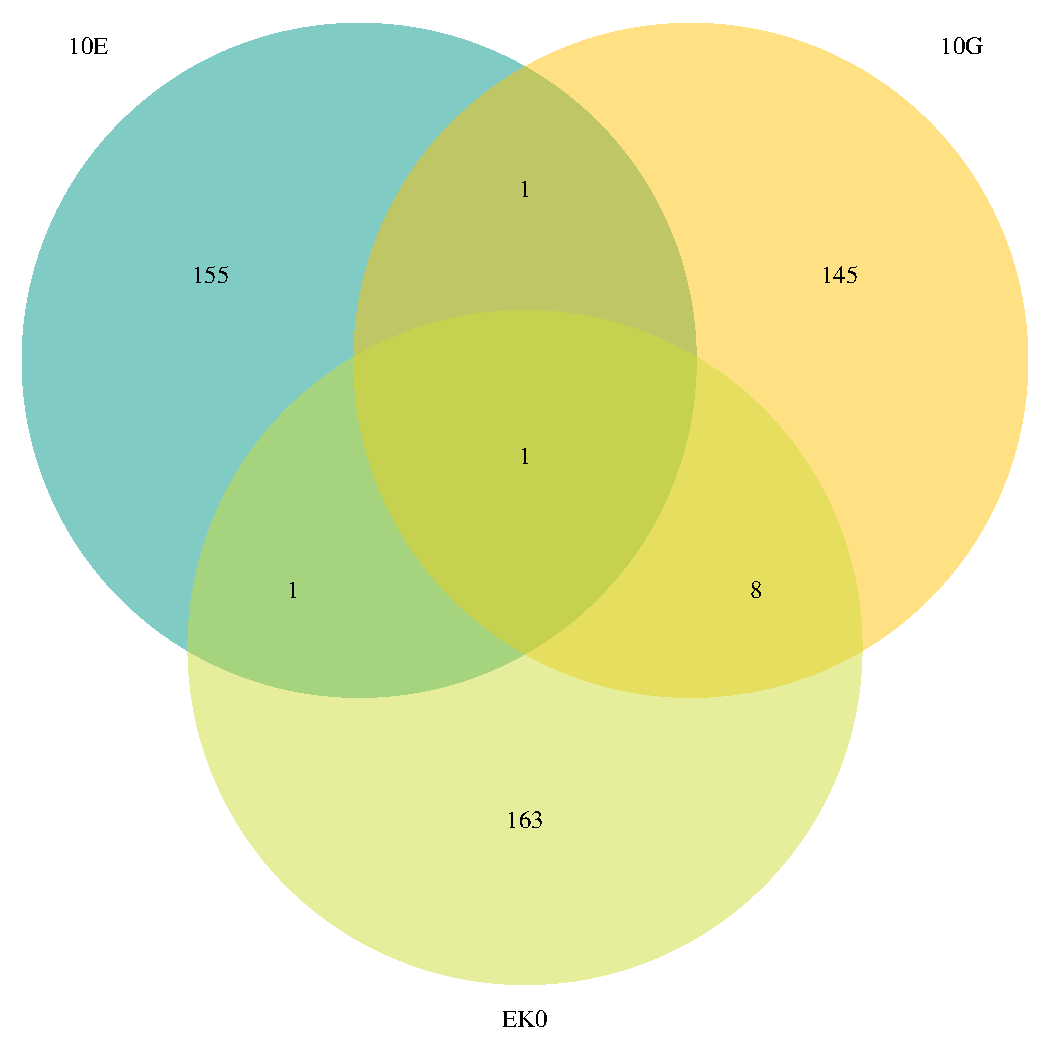
\includegraphics[width=1\linewidth,height=.4\textheight]{figure/minimal-venn_t1_3fc_up_venn-1} 

}



\end{knitrout}
\begin{knitrout}
\definecolor{shadecolor}{rgb}{0.969, 0.969, 0.969}\color{fgcolor}

{\centering 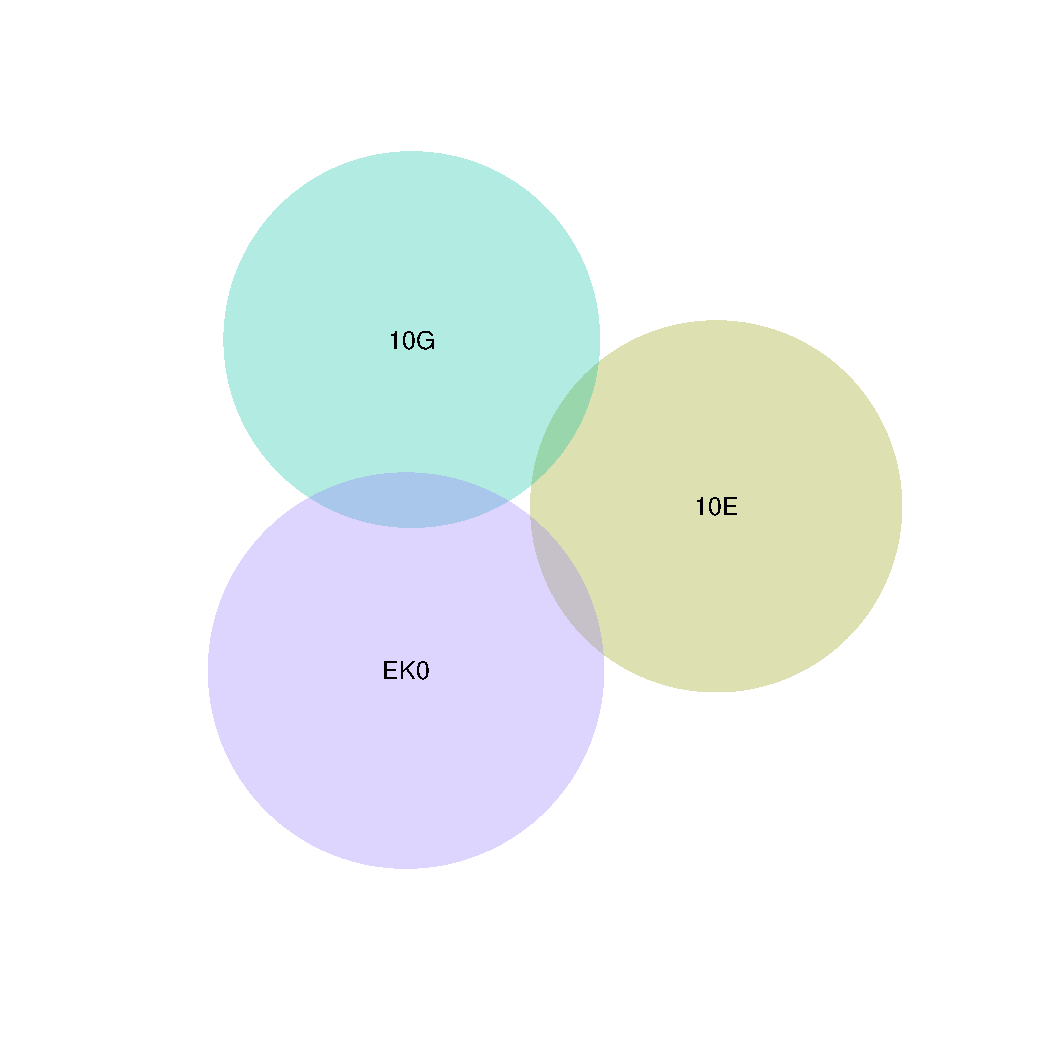
\includegraphics[width=1\linewidth,height=.4\textheight]{figure/minimal-venn_t1_3fc_up_euler-1} 

}



\end{knitrout}
\clearpage
\subsubsection{Down-regulated}

\begin{knitrout}
\definecolor{shadecolor}{rgb}{0.969, 0.969, 0.969}\color{fgcolor}\begin{kframe}
\begin{verbatim}
## (polygon[GRID.polygon.49], polygon[GRID.polygon.50], polygon[GRID.polygon.51], polygon[GRID.polygon.52], polygon[GRID.polygon.53], polygon[GRID.polygon.54], text[GRID.text.55], text[GRID.text.56], text[GRID.text.57], text[GRID.text.58], text[GRID.text.59], text[GRID.text.60], text[GRID.text.61], text[GRID.text.62], text[GRID.text.63])
\end{verbatim}
\end{kframe}

{\centering 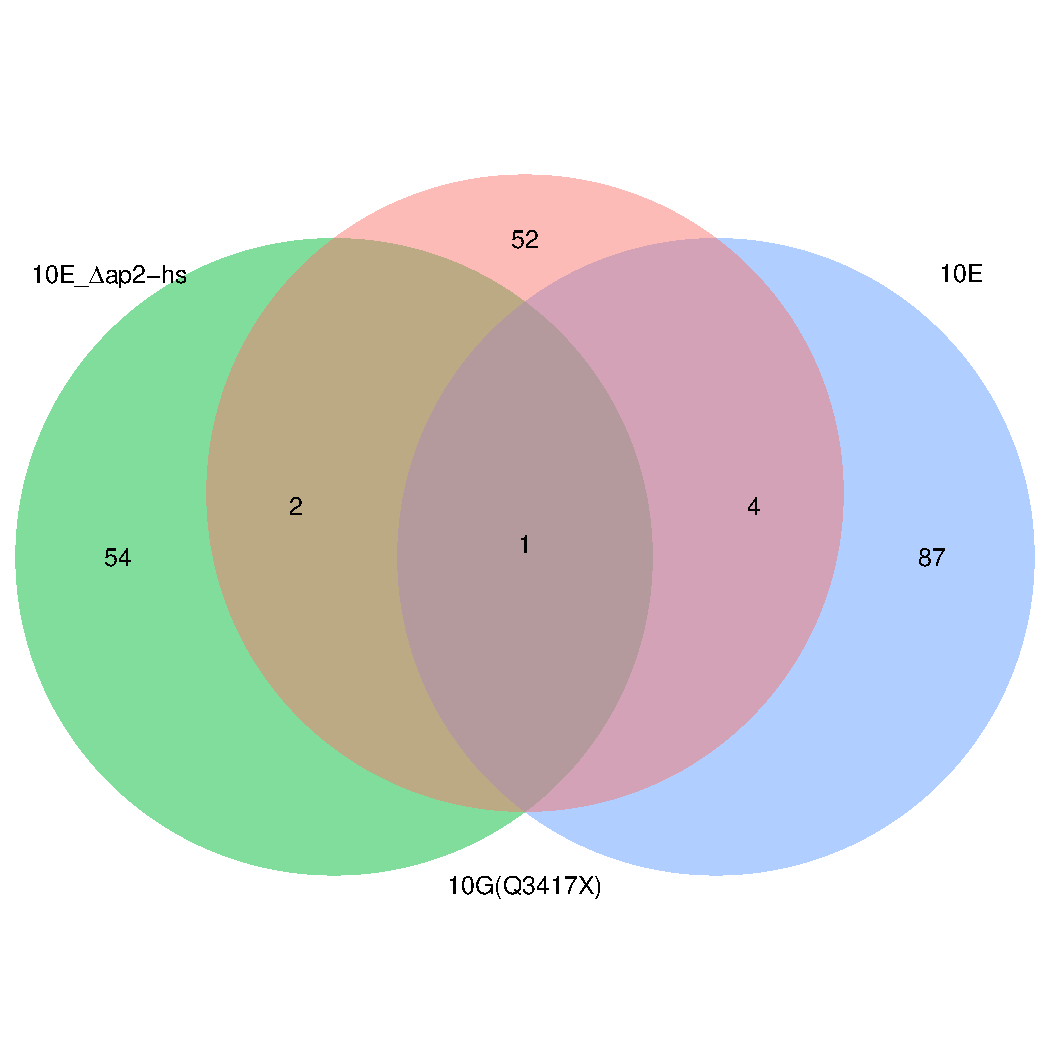
\includegraphics[width=1\linewidth,height=.4\textheight]{figure/minimal-venn_t1_3fc_down_venn-1} 

}



\end{knitrout}
\begin{knitrout}
\definecolor{shadecolor}{rgb}{0.969, 0.969, 0.969}\color{fgcolor}

{\centering 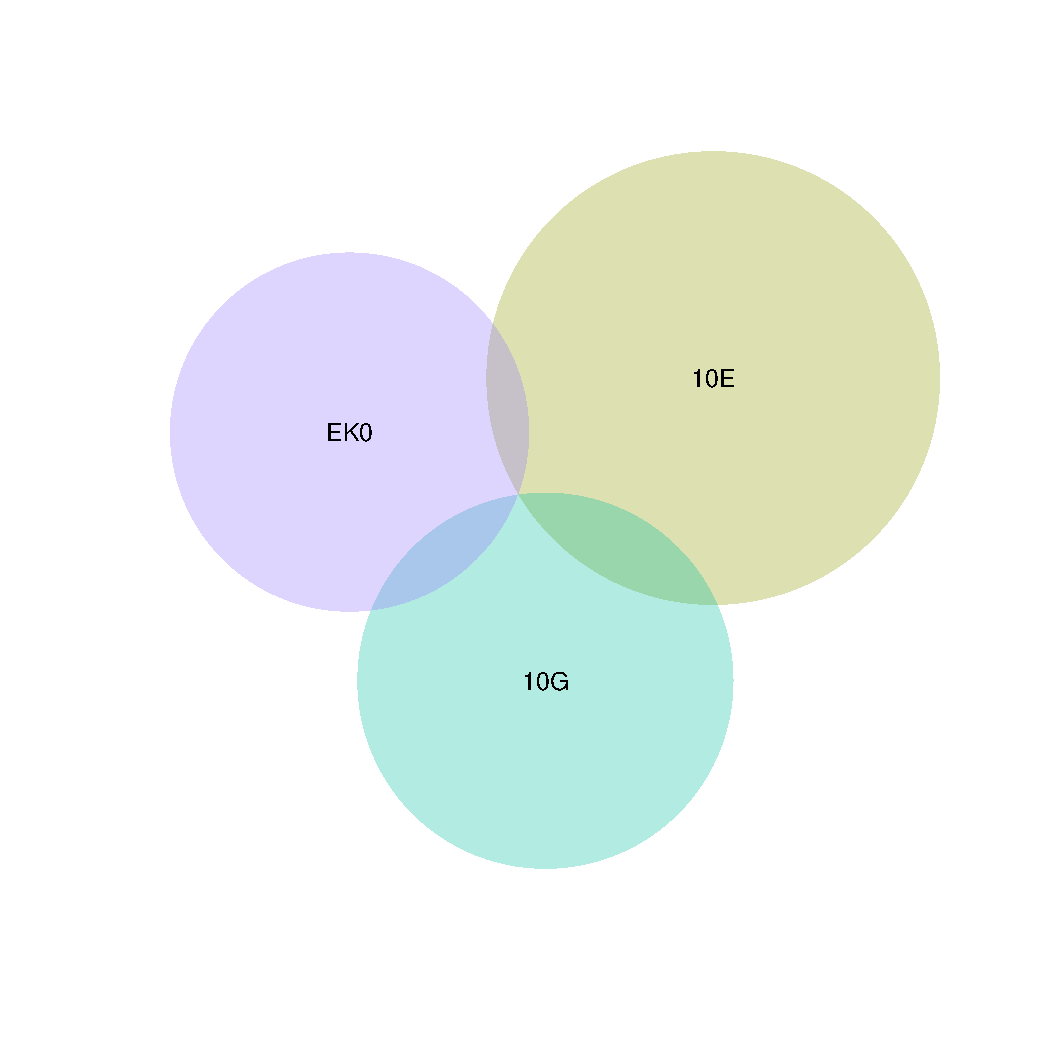
\includegraphics[width=1\linewidth,height=.4\textheight]{figure/minimal-venn_t1_3fc_down_euler-1} 

}



\end{knitrout}
\clearpage

\subsection{Max.FC T2 $>3$ FC}
\subsubsection{Up-regulated}

\begin{knitrout}
\definecolor{shadecolor}{rgb}{0.969, 0.969, 0.969}\color{fgcolor}\begin{kframe}
\begin{verbatim}
## (polygon[GRID.polygon.64], polygon[GRID.polygon.65], polygon[GRID.polygon.66], polygon[GRID.polygon.67], polygon[GRID.polygon.68], polygon[GRID.polygon.69], text[GRID.text.70], text[GRID.text.71], text[GRID.text.72], text[GRID.text.73], text[GRID.text.74], text[GRID.text.75], text[GRID.text.76], text[GRID.text.77], text[GRID.text.78], text[GRID.text.79])
\end{verbatim}
\end{kframe}

{\centering 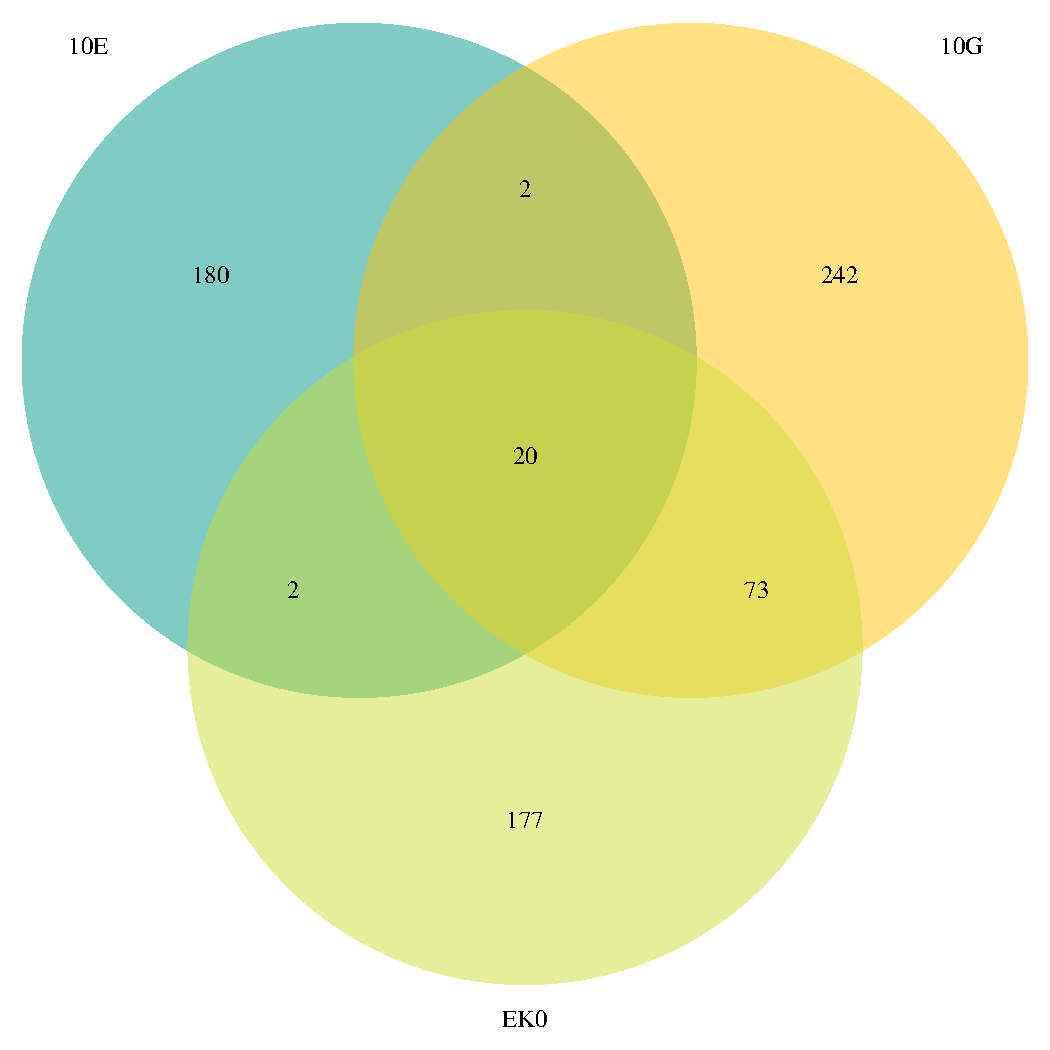
\includegraphics[width=1\linewidth,height=.4\textheight]{figure/minimal-venn_t2_3fc_up_venn-1} 

}



\end{knitrout}
\begin{knitrout}
\definecolor{shadecolor}{rgb}{0.969, 0.969, 0.969}\color{fgcolor}

{\centering 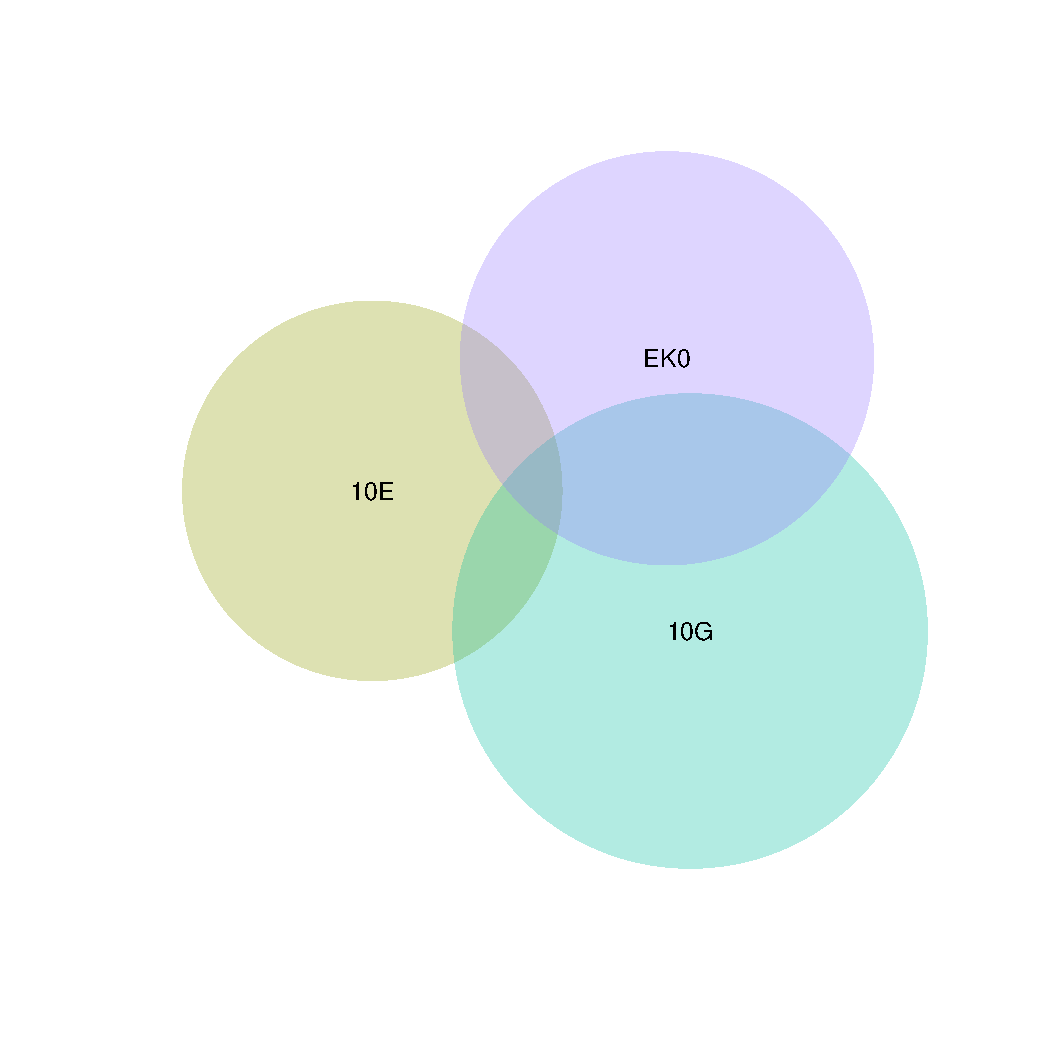
\includegraphics[width=1\linewidth,height=.4\textheight]{figure/minimal-venn_t2_3fc_up_euler-1} 

}



\end{knitrout}
\clearpage
\subsubsection{Down-Regulated}

\begin{knitrout}
\definecolor{shadecolor}{rgb}{0.969, 0.969, 0.969}\color{fgcolor}\begin{kframe}
\begin{verbatim}
## (polygon[GRID.polygon.80], polygon[GRID.polygon.81], polygon[GRID.polygon.82], polygon[GRID.polygon.83], polygon[GRID.polygon.84], polygon[GRID.polygon.85], text[GRID.text.86], text[GRID.text.87], text[GRID.text.88], text[GRID.text.89], text[GRID.text.90], text[GRID.text.91], text[GRID.text.92], text[GRID.text.93], text[GRID.text.94], text[GRID.text.95])
\end{verbatim}
\end{kframe}

{\centering 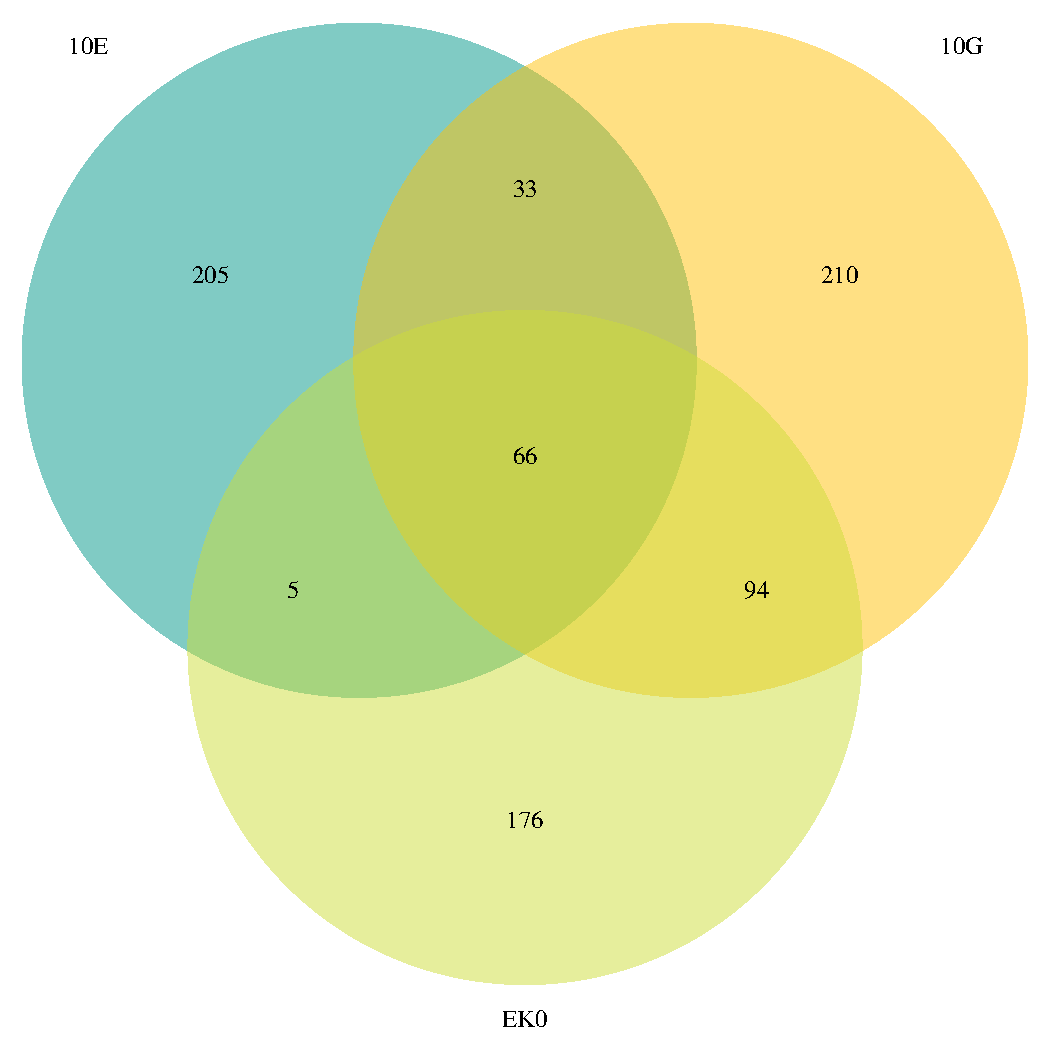
\includegraphics[width=1\linewidth,height=.4\textheight]{figure/minimal-venn_t2_3fc_down_venn-1} 

}



\end{knitrout}
\begin{knitrout}
\definecolor{shadecolor}{rgb}{0.969, 0.969, 0.969}\color{fgcolor}

{\centering 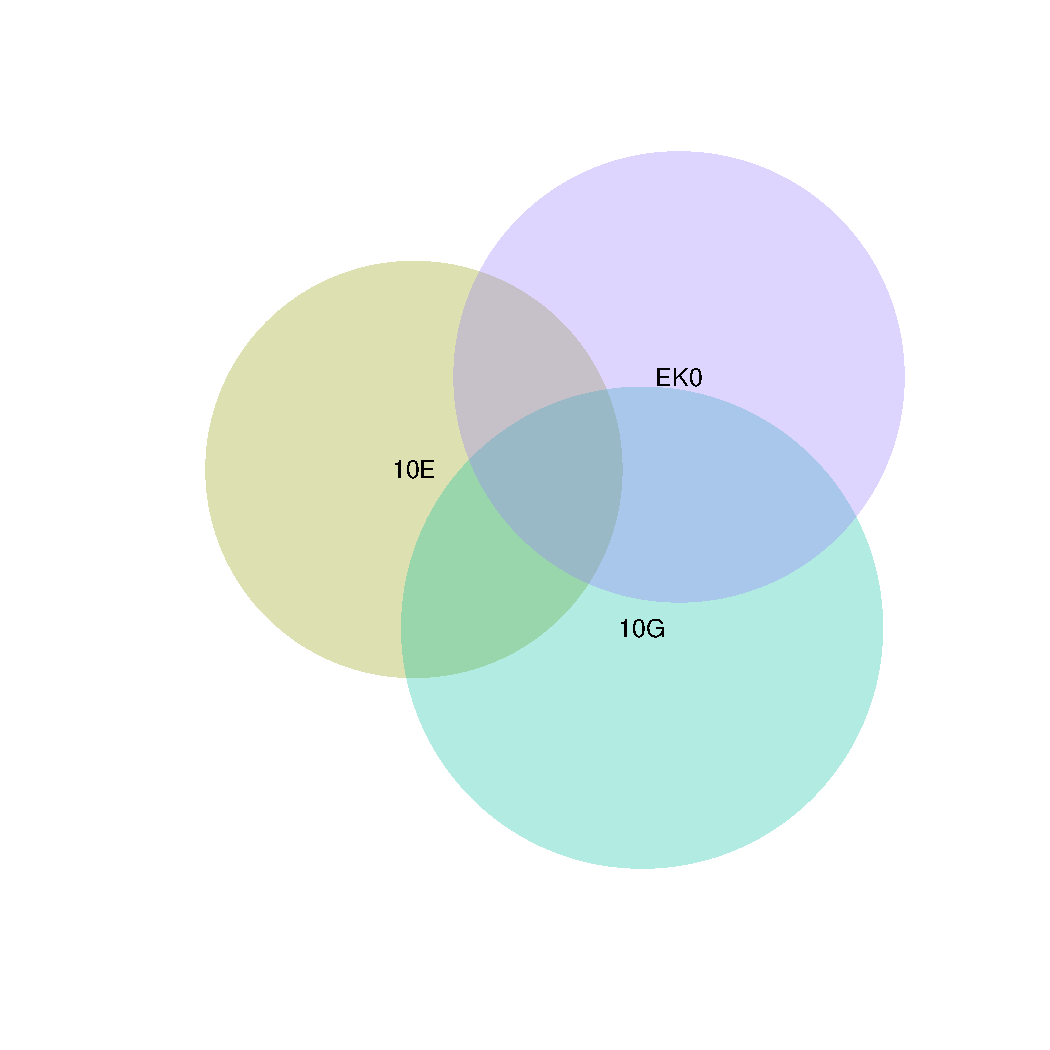
\includegraphics[width=1\linewidth,height=.4\textheight]{figure/minimal-venn_t2_3fc_down_euler-1} 

}



\end{knitrout}
\clearpage

\subsection{Max.FC T3 $>3$ FC}
\subsubsection{Up-regulated}

\begin{knitrout}
\definecolor{shadecolor}{rgb}{0.969, 0.969, 0.969}\color{fgcolor}\begin{kframe}
\begin{verbatim}
## (polygon[GRID.polygon.96], polygon[GRID.polygon.97], polygon[GRID.polygon.98], polygon[GRID.polygon.99], polygon[GRID.polygon.100], polygon[GRID.polygon.101], text[GRID.text.102], text[GRID.text.103], text[GRID.text.104], text[GRID.text.105], text[GRID.text.106], text[GRID.text.107], text[GRID.text.108], text[GRID.text.109], text[GRID.text.110], text[GRID.text.111])
\end{verbatim}
\end{kframe}

{\centering 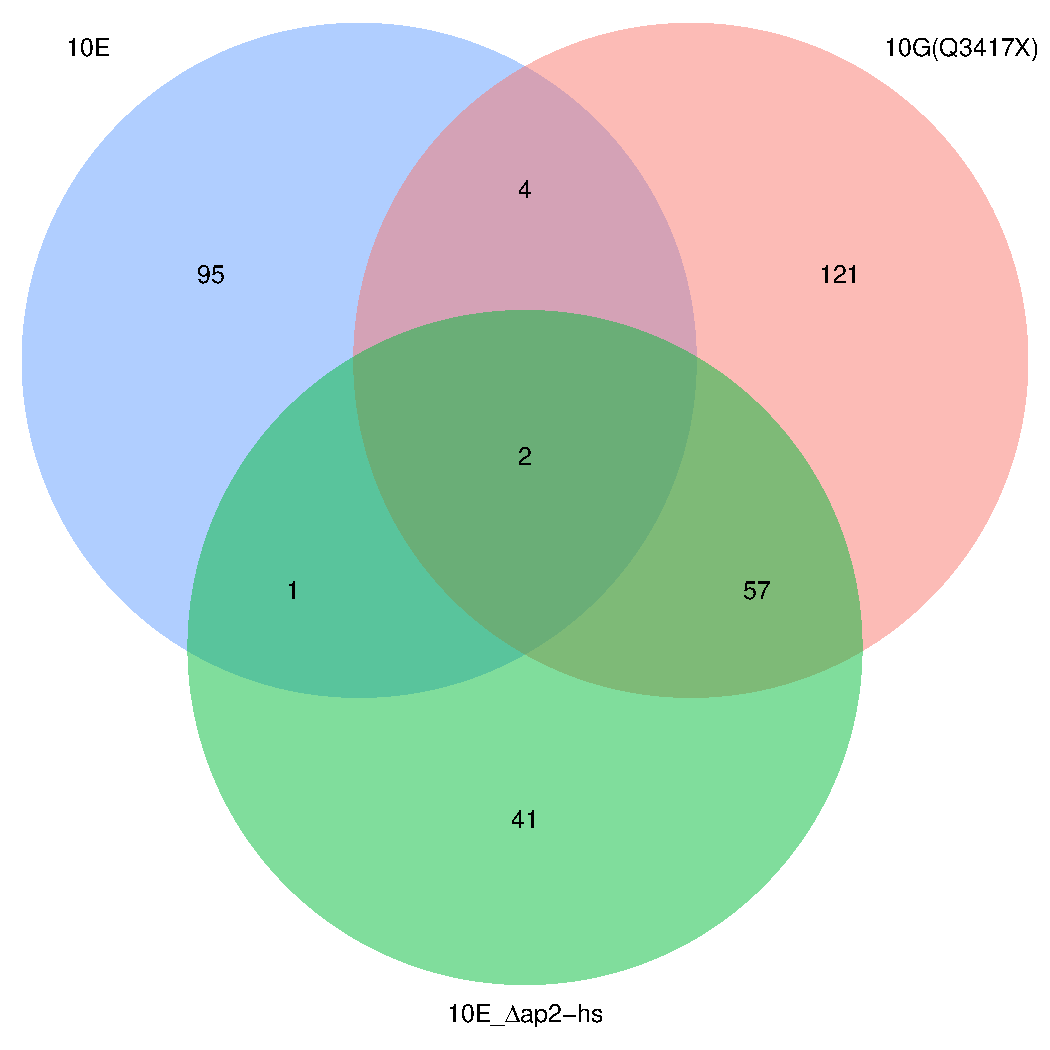
\includegraphics[width=1\linewidth,height=.4\textheight]{figure/minimal-venn_t3_3fc_up_venn-1} 

}



\end{knitrout}
\begin{knitrout}
\definecolor{shadecolor}{rgb}{0.969, 0.969, 0.969}\color{fgcolor}

{\centering 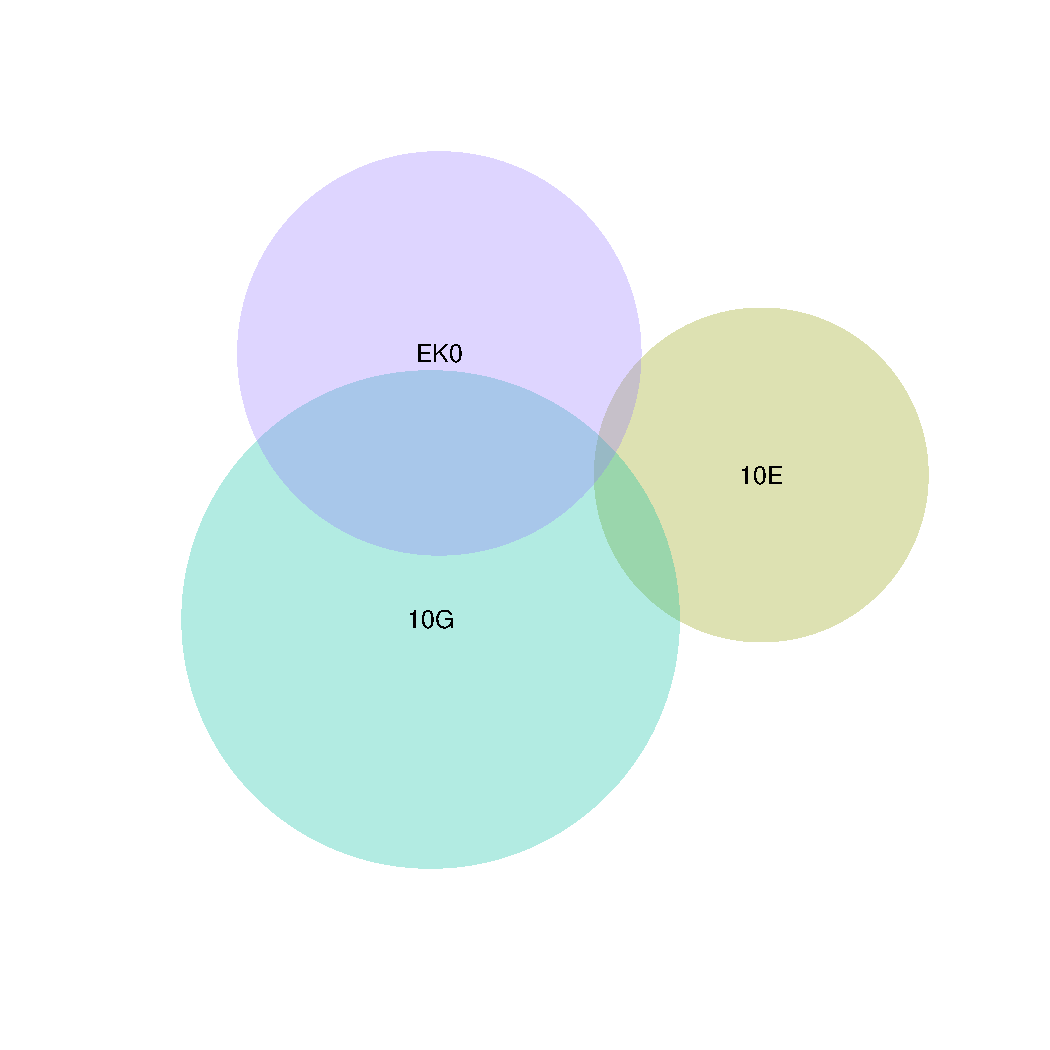
\includegraphics[width=1\linewidth,height=.4\textheight]{figure/minimal-venn_t3_3fc_up_euler-1} 

}



\end{knitrout}
\clearpage
\subsubsection{Down-Regulated}

\begin{knitrout}
\definecolor{shadecolor}{rgb}{0.969, 0.969, 0.969}\color{fgcolor}\begin{kframe}
\begin{verbatim}
## (polygon[GRID.polygon.112], polygon[GRID.polygon.113], polygon[GRID.polygon.114], polygon[GRID.polygon.115], polygon[GRID.polygon.116], polygon[GRID.polygon.117], text[GRID.text.118], text[GRID.text.119], text[GRID.text.120], text[GRID.text.121], text[GRID.text.122], text[GRID.text.123], text[GRID.text.124], text[GRID.text.125], text[GRID.text.126], text[GRID.text.127])
\end{verbatim}
\end{kframe}

{\centering 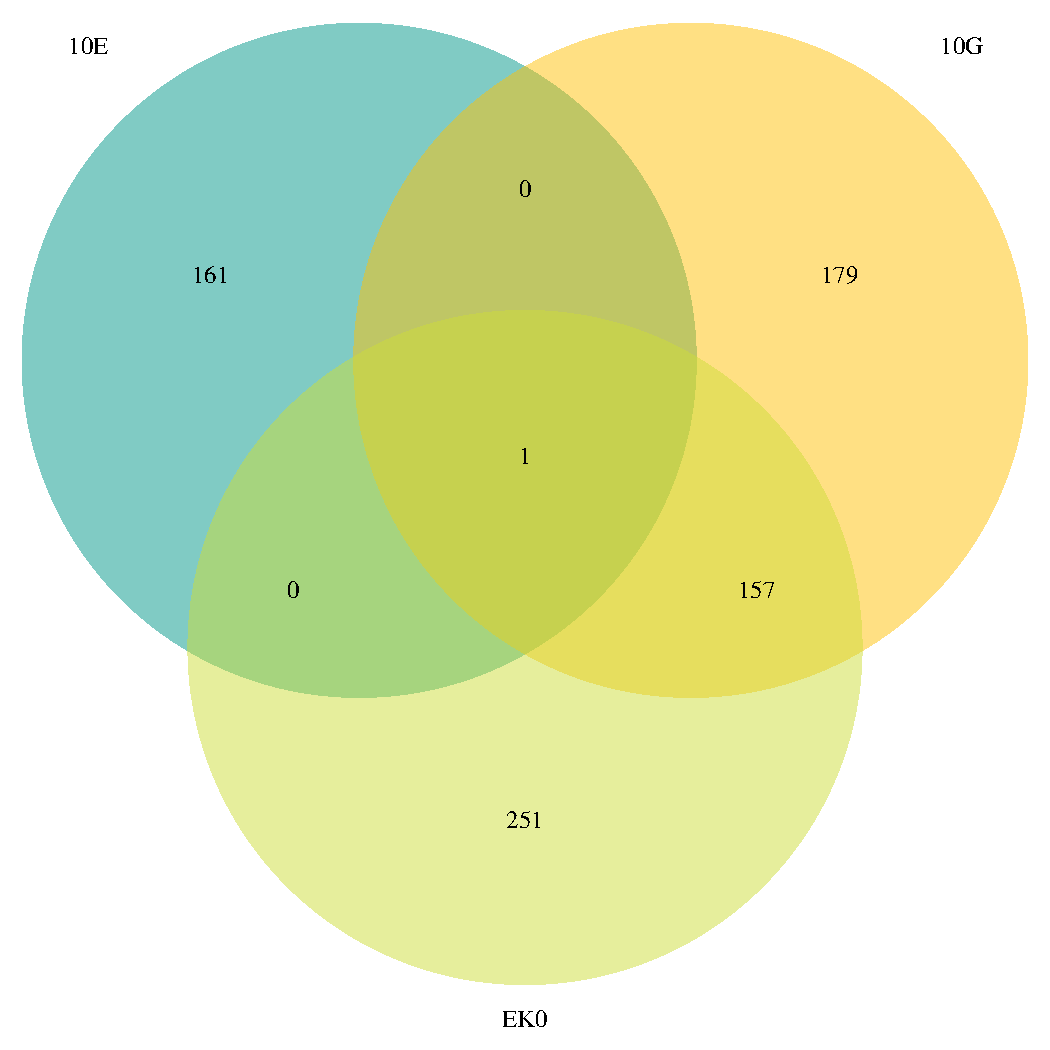
\includegraphics[width=1\linewidth,height=.4\textheight]{figure/minimal-venn_t3_3fc_down_venn-1} 

}



\end{knitrout}
\begin{knitrout}
\definecolor{shadecolor}{rgb}{0.969, 0.969, 0.969}\color{fgcolor}

{\centering 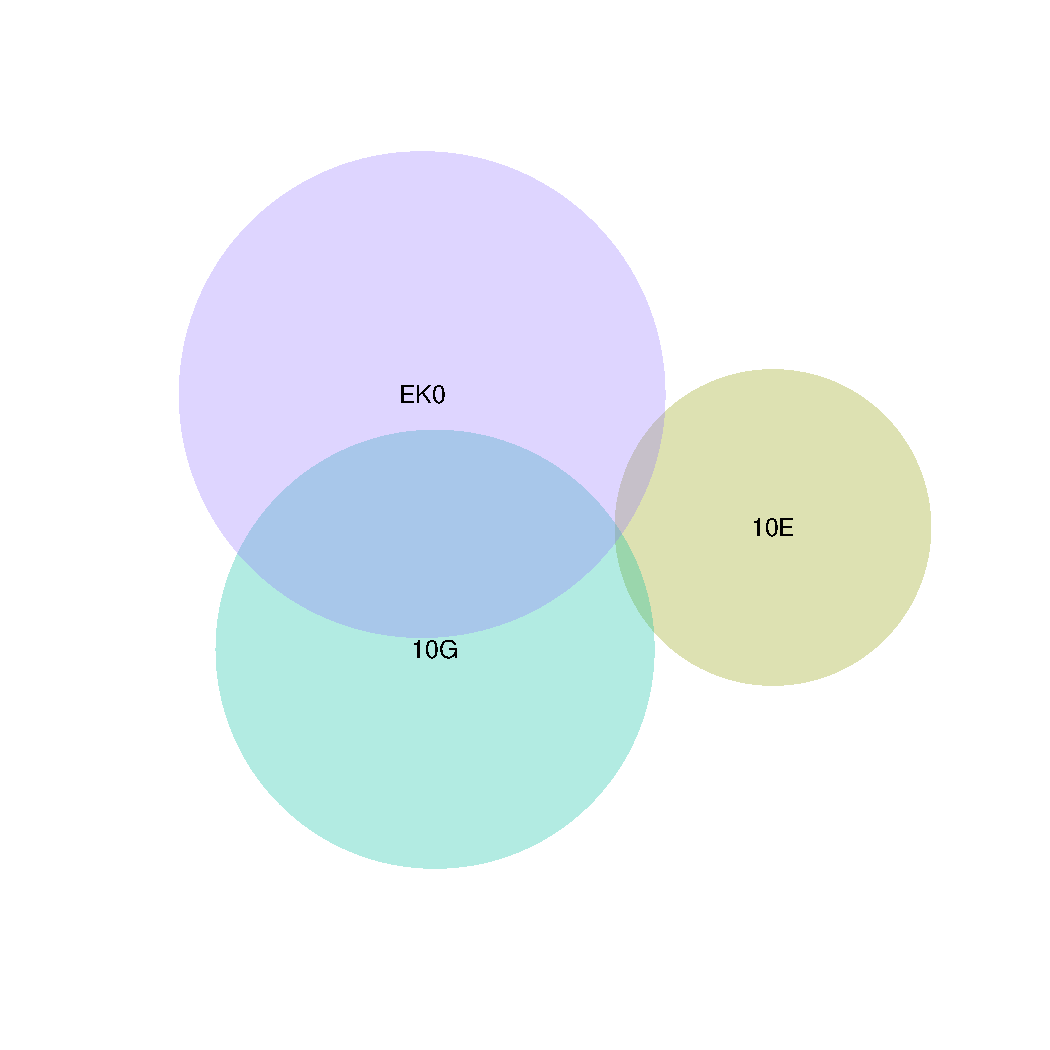
\includegraphics[width=1\linewidth,height=.4\textheight]{figure/minimal-venn_t3_3fc_down_euler-1} 

}



\end{knitrout}
\clearpage



%%%%------------------------------------------------CUSTOM------------------------------------------------%%%%



\section{Example Custom Plot}
\begin{knitrout}
\definecolor{shadecolor}{rgb}{0.969, 0.969, 0.969}\color{fgcolor}

{\centering 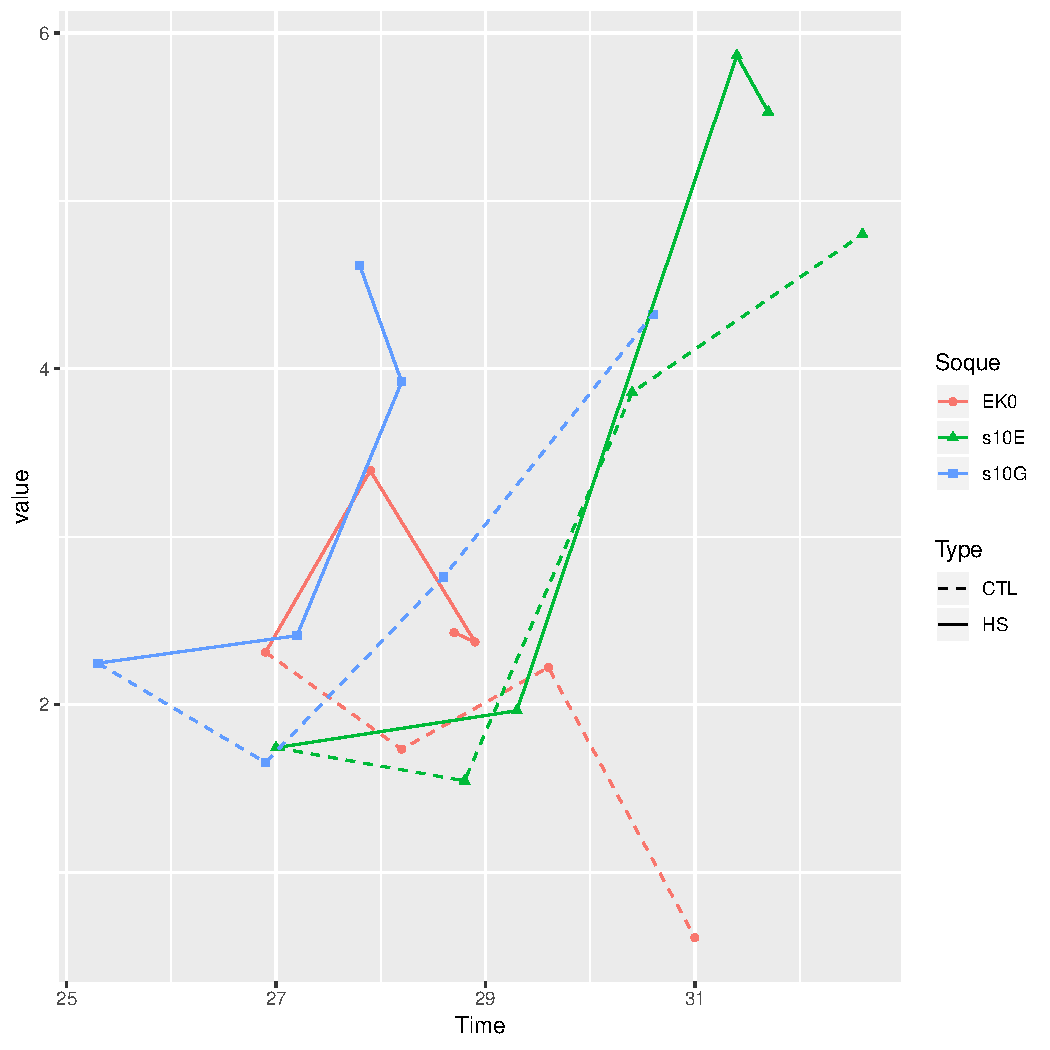
\includegraphics[width=1\linewidth]{figure/minimal-custom_plots-1} 

}



\end{knitrout}
\clearpage



%%%%------------------------------------------------HEATMAPS------------------------------------------------%%%%


\section{Heat maps}
\subsection{Top FC separated}
\begin{knitrout}
\definecolor{shadecolor}{rgb}{0.969, 0.969, 0.969}\color{fgcolor}

{\centering 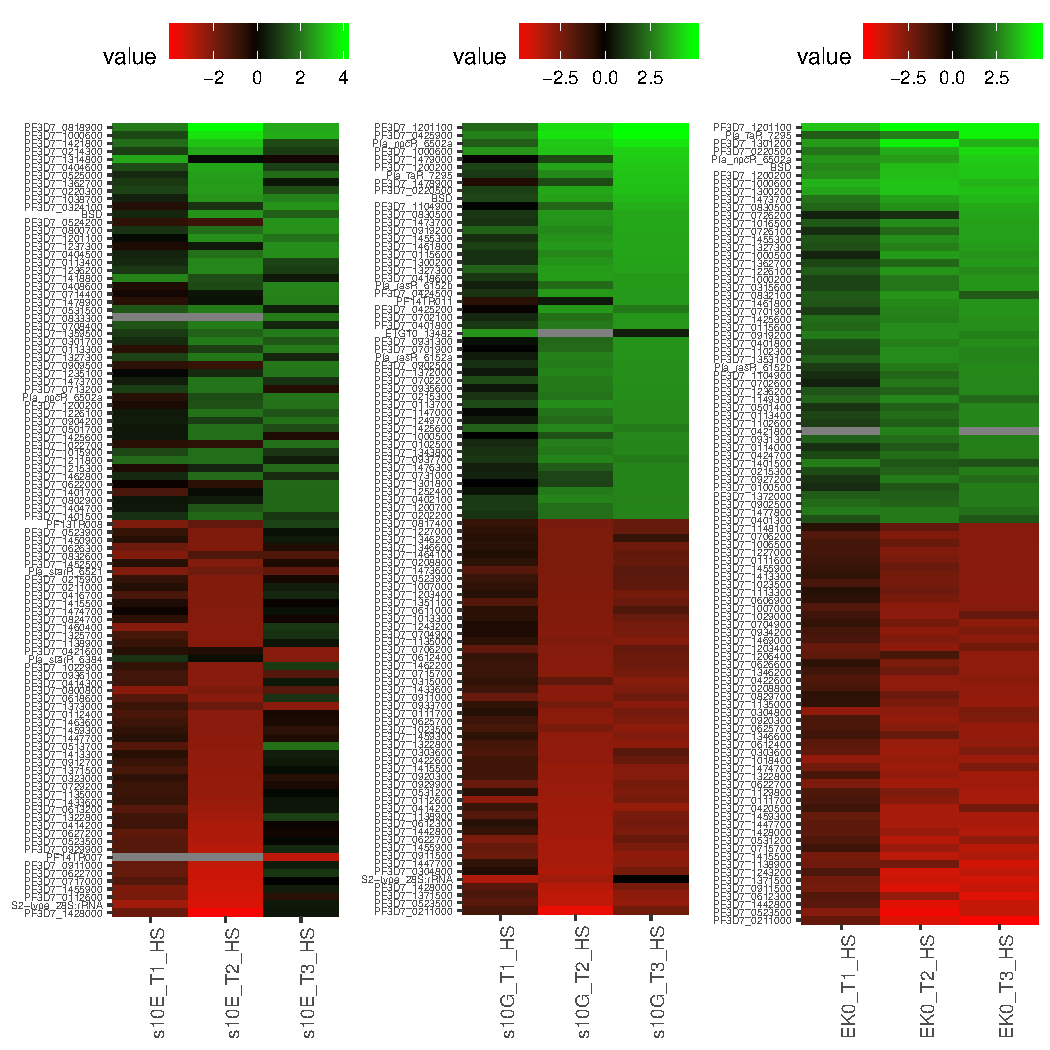
\includegraphics[width=1\linewidth]{figure/minimal-heatmaps-1} 

}



\end{knitrout}
\clearpage
\subsection{Top FC in 10E, across strains, ordered}
\begin{knitrout}
\definecolor{shadecolor}{rgb}{0.969, 0.969, 0.969}\color{fgcolor}

{\centering 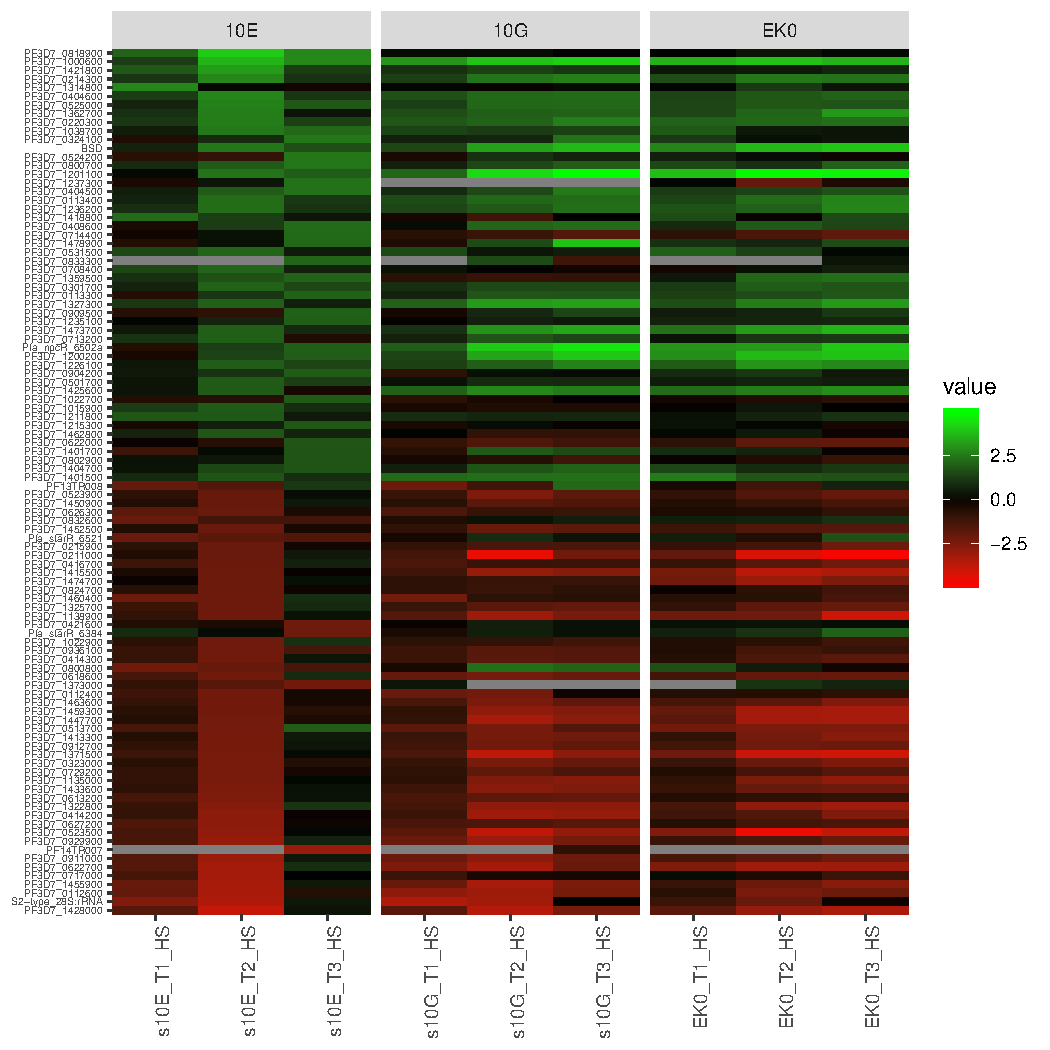
\includegraphics[width=1\linewidth]{figure/minimal-heatmap_all_facet-1} 

}



\end{knitrout}
\clearpage
\subsection{Top FC in 10E, across strains, clustered}
\begin{knitrout}
\definecolor{shadecolor}{rgb}{0.969, 0.969, 0.969}\color{fgcolor}

{\centering 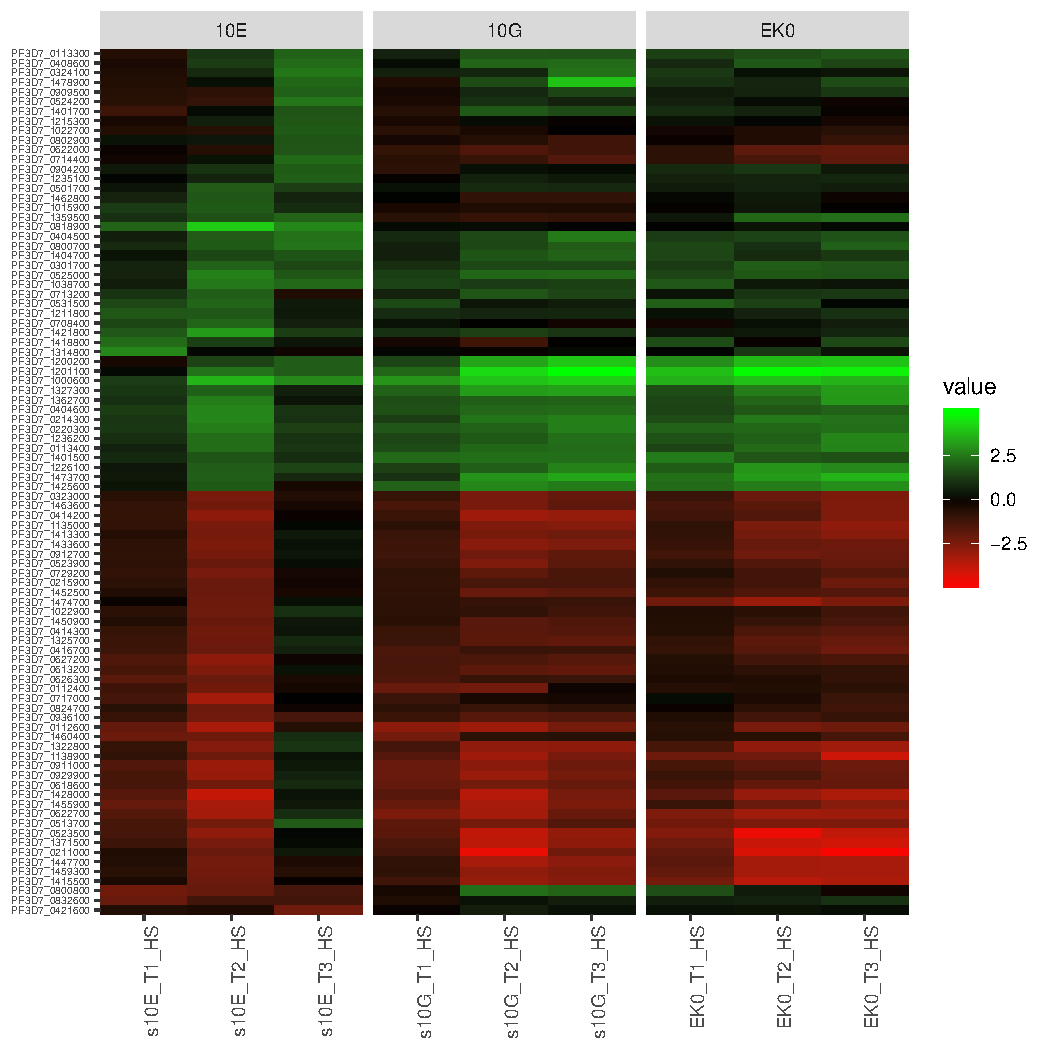
\includegraphics[width=1\linewidth]{figure/minimal-heatmap_all_10E_clustered-1} 

}



\end{knitrout}
\clearpage
\subsection{FC $>$6 in all strains combined, clustered}
\begin{knitrout}
\definecolor{shadecolor}{rgb}{0.969, 0.969, 0.969}\color{fgcolor}

{\centering 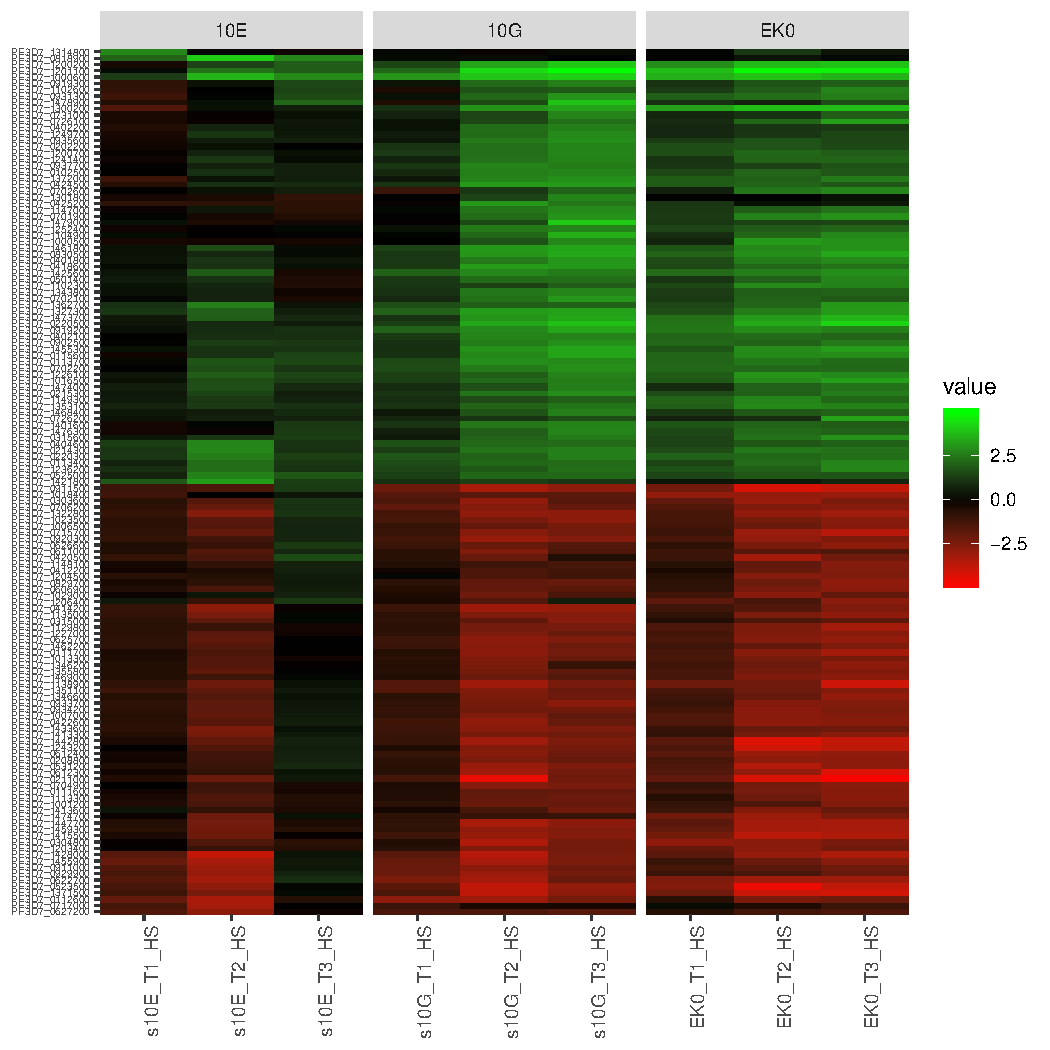
\includegraphics[width=1\linewidth]{figure/minimal-heatmap_all_clustered-1} 

}



\end{knitrout}



%%%%------------------------------------------------PCA------------------------------------------------%%%%



\clearpage
\section{Principal Component Analysis}
\begin{knitrout}
\definecolor{shadecolor}{rgb}{0.969, 0.969, 0.969}\color{fgcolor}

{\centering 
\includegraphics[width=1\linewidth]{figure/minimal-pcas-1} 
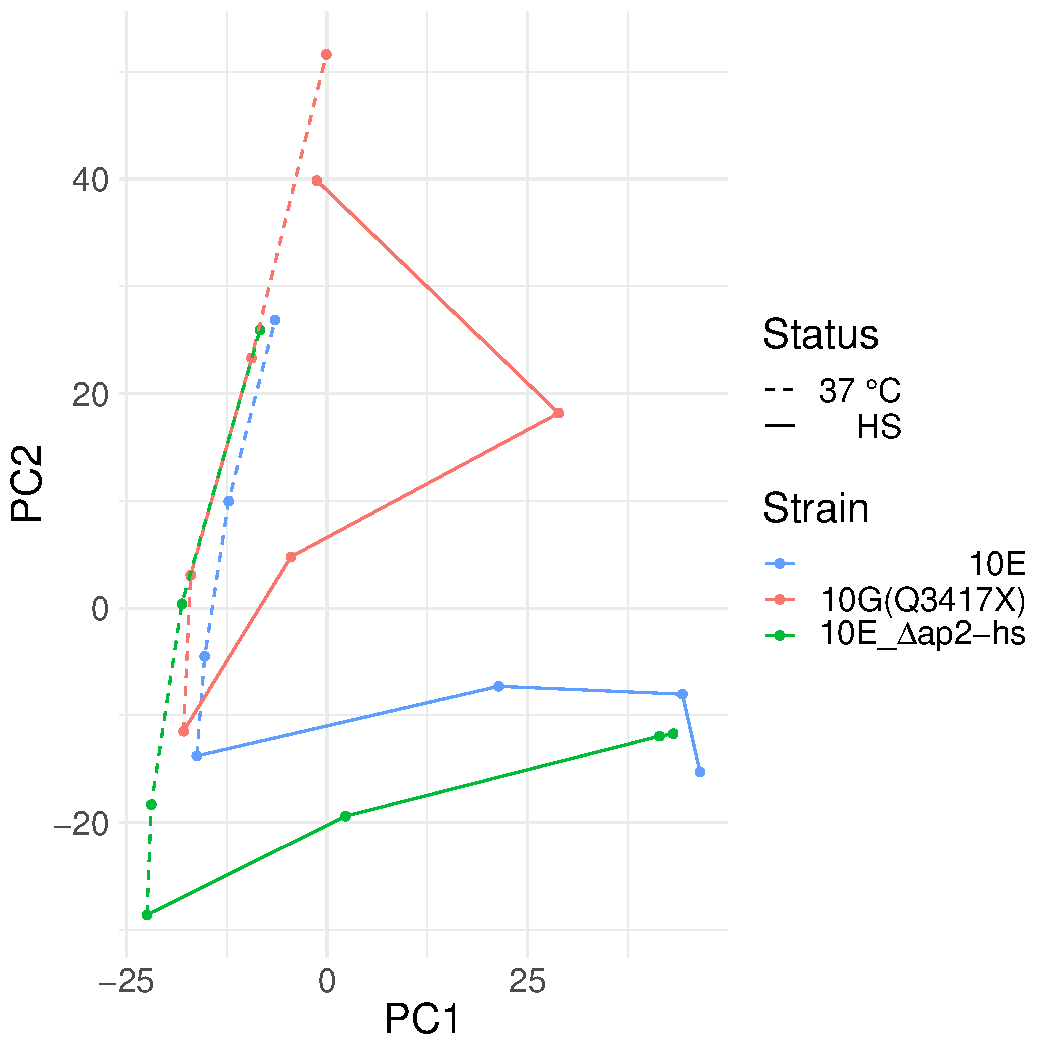
\includegraphics[width=1\linewidth]{figure/minimal-pcas-2} 

}



\end{knitrout}

\end{document}










